% ******************************* PhD Thesis Template **************************
% Please have a look at the README.md file for info on how to use the template

\documentclass[a4paper,12pt,times,numbered,print,index]{Classes/PhDThesisPSnPDF}
% ********************************** Preamble **********************************
% Preamble: Contains packages and user-defined commands and settings
% ******************************************************************************
% ****************************** Custom Margin *********************************

% Add `custommargin' in the document class options to use this section
% Set {innerside margin / outerside margin / topmargin / bottom margin}  and
% other page dimensions
\ifsetCustomMargin
  \RequirePackage[left=37mm,right=30mm,top=35mm,bottom=30mm]{geometry}
  \setFancyHdr % To apply fancy header after geometry package is loaded
\fi

% *****************************************************************************
% ******************* Fonts (like different typewriter fonts etc.)*************

% Add `customfont' in the document class option to use this section

\ifsetCustomFont
  % Set your custom font here and use `customfont' in options. Leave empty to
  % load computer modern font (default LaTeX font).
  \RequirePackage{helvet}
\fi

% *****************************************************************************
% **************************** Custom Packages ********************************

% ************************* Algorithms and Pseudocode **************************

%\usepackage{algpseudocode}


% ********************Captions and Hyperreferencing / URL **********************

% Captions: This makes captions of figures use a boldfaced small font.
%\RequirePackage[small,bf]{caption}

\RequirePackage[labelsep=space,tableposition=top]{caption}
\renewcommand{\figurename}{Fig.} %to support older versions of captions.sty


% *************************** Graphics and figures *****************************

%\usepackage{rotating}
%\usepackage{wrapfig}

% Uncomment the following two lines to force Latex to place the figure.
% Use [H] when including graphics. Note 'H' instead of 'h'
%\usepackage{float}
%\restylefloat{figure}

% Subcaption package is also available in the sty folder you can use that by
% uncommenting the following line
% This is for people stuck with older versions of texlive
%\usepackage{sty/caption/subcaption}
\usepackage{subcaption}

% ********************************** Tables ************************************
\usepackage{booktabs} % For professional looking tables
\usepackage{multirow}

\usepackage{multicol}
%\usepackage{longtable}
%\usepackage{tabularx}


% ***************************** Math and SI Units ******************************

\usepackage{amsfonts}
\usepackage{amsmath}
\usepackage{amssymb}
%\usepackage{siunitx} % use this package module for SI units


% ******************************* Line Spacing *********************************

% Choose linespacing as appropriate. Default is one-half line spacing as per the
% University guidelines

% \doublespacing
% \onehalfspacing
% \singlespacing


% ************************ Formatting / Footnote *******************************

% Don't break enumeration (etc.) across pages in an ugly manner (default 10000)
%\clubpenalty=500
%\widowpenalty=500

%\usepackage[perpage]{footmisc} %Range of footnote options


% *****************************************************************************
% *************************** Bibliography  and References ********************

%\usepackage{cleveref} %Referencing without need to explicitly state fig /table

% Add `custombib' in the document class option to use this section
\ifuseCustomBib
   \RequirePackage[square, sort, numbers, authoryear]{natbib} % CustomBib

% If you would like to use biblatex for your reference management, as opposed to the default `natbibpackage` pass the option `custombib` in the document class. Comment out the previous line to make sure you don't load the natbib package. Uncomment the following lines and specify the location of references.bib file

%\RequirePackage[backend=biber, style=numeric-comp, citestyle=numeric, sorting=nty, natbib=true]{biblatex}
%\bibliography{References/references} %Location of references.bib only for biblatex

\fi

% changes the default name `Bibliography` -> `References'
\renewcommand{\bibname}{References}


% *****************************************************************************
% *************** Changing the Visual Style of Chapter Headings ***************
% This section on visual style is from https://github.com/cambridge/thesis

% Uncomment the section below. Requires titlesec package.

%\RequirePackage{titlesec}
%\newcommand{\PreContentTitleFormat}{\titleformat{\chapter}[display]{\scshape\Large}
%{\Large\filleft{\chaptertitlename} \Huge\thechapter}
%{1ex}{}
%[\vspace{1ex}\titlerule]}
%\newcommand{\ContentTitleFormat}{\titleformat{\chapter}[display]{\scshape\huge}
%{\Large\filleft{\chaptertitlename} \Huge\thechapter}{1ex}
%{\titlerule\vspace{1ex}\filright}
%[\vspace{1ex}\titlerule]}
%\newcommand{\PostContentTitleFormat}{\PreContentTitleFormat}
%\PreContentTitleFormat


% ******************************************************************************
% ************************* User Defined Commands ******************************
% ******************************************************************************

% *********** To change the name of Table of Contents / LOF and LOT ************

%\renewcommand{\contentsname}{My Table of Contents}
%\renewcommand{\listfigurename}{My List of Figures}
%\renewcommand{\listtablename}{My List of Tables}


% ********************** TOC depth and numbering depth *************************

\setcounter{secnumdepth}{2}
\setcounter{tocdepth}{2}









\usepackage{siunitx}
\usepackage{wrapfig}

% ************************ Thesis Information & Meta-data **********************
% Thesis title and author information, refernce file for biblatex
% ************************ Thesis Information & Meta-data **********************
%% The title of the thesis
\title{Teo: a mobile robot as support for the treatment of children affected by Autistic Spectrum Disorder}
%\texorpdfstring is used for PDF metadata. Usage:
%\texorpdfstring{LaTeX_Version}{PDF Version (non-latex)} eg.,
%\texorpdfstring{$sigma$}{sigma}

%% Subtitle (Optional)
%\subtitle{Using the CUED template}

%% The full name of the author
\author{Author: Matteo Lucchelli [838107] \\ Supervisor: Andrea Bonarini}

%% Department (eg. Department of Engineering, Maths, Physics)
\dept{ Dipartimento di Elettronica, Informazione e Bioingegneria (DEIB)}

%% University and Crest
\university{Politecnico di Milano}
\crest{
\includegraphics[width=0.30\textwidth]{polimi}}

%% You can redefine the submission text:
% Default as per the University guidelines:
% ``This dissertation is submitted for the degree of''
%\renewcommand{\submissiontext}{change the default text here if needed}

%% Full title of the Degree
\degree{Master Degree in Computer Science and Engineering}

%% College affiliation (optional)
\college{Artificial Intelligence and Robotics Laboratory (AIRlab)}

%% Submission date
% Default isà set as {\monthname[\the\month]\space\the\year}
%\degreedate{September 2014} 

%% Meta information
\subject{LaTeX} \keywords{{LaTeX} {PhD Thesis} {Engineering} {Politecnico di Milano}}


% ***************************** Abstract Separate ******************************
% To printout only the titlepage and the abstract with the PhD title and the
% author name for submission to the Student Registry, use the `abstract' option in
% the document class.

\ifdefineAbstract
 \pagestyle{empty}
 \includeonly{Declaration/declaration, Abstract/abstract}
\fi

% ***************************** Chapter Mode ***********************************
% The chapter mode allows user to only print particular chapters with references
% Title, Contents, Frontmatter are disabled by default
% Useful option to review a particular chapter or to send it to supervisior.
% To use choose `chapter' option in the document class

%\ifdefineChapter
% \includeonly{Chapter3/chapter3}
%\fi

% ******************************** Front Matter ********************************
\begin{document}

\frontmatter

\begin{titlepage}
  \maketitle
\end{titlepage}


% ******************************* Thesis Dedidcation ********************************

\begin{dedication} 

I would like to dedicate this thesis to my loving robots ...

\end{dedication}


% ************************** Thesis Acknowledgements *****************************

\begin{acknowledgements}      


And I would like to acknowledge ...


\end{acknowledgements}

% ************************** Thesis Abstract *****************************
% Use `abstract' as an option in the document class to print only the titlepage and the abstract.
\begin{abstract}

\end{abstract}


% *********************** Adding TOC and List of Figures ***********************

\tableofcontents

\listoffigures

\listoftables

% \printnomencl[space] space can be set as 2em between symbol and description
%\printnomencl[3em]

%\printnomencl

% ******************************** Main Matter *********************************
\mainmatter

%*******************************************************************************
%*********************************** First Chapter *****************************
%*******************************************************************************
\chapter{Introduction}  %Title of the First Chapter
\label{chapter1}
\ifpdf
    \graphicspath{{Chapter1/Figs/Raster/}{Chapter1/Figs/PDF/}{Chapter1/Figs/}}
\else
    \graphicspath{{Chapter1/Figs/Vector/}{Chapter1/Figs/}}
\fi


%********************************** %First Section  **************************************

\section{Inquadramento generale}
La prima parte contiene una frase che spiega l'area generale dove si svolge il lavoro; una che spiega la sottoarea pi\`u specifica dove si svolge il lavoro e la terza, che dovrebbe cominciare con le seguenti parole ``lo scopo della tesi \`e \dots'', illustra l'obbiettivo del lavoro. Poi vi devono essere una o due frasi che contengano una breve spiegazione di cosa e come \`e stato fatto, delle attivit\`a  sperimentali, dei risultati ottenuti con una valutazione e degli sviluppi futuri. La prima parte deve essere circa una facciata e mezza o due.
The ultimate goal is to help
children with autism in making sense of the world, assisted by computer and robotic technology.

\section{Breve descrizione del lavoro}
La seconda parte deve essere una esplosione della prima e deve quindi mostrare in maniera pi\`u esplicita l'area dove si svolge il lavoro, le fonti bibliografiche pi\`u importanti su cui si fonda il lavoro in maniera sintetica (una pagina) evidenziando i lavori in letteratura che presentano attinenza con il lavoro affrontato in modo da mostrare da dove e perch\'e \`e sorta la tematica di studio. Poi si mostrano esplicitamente le realizzazioni, le direttive future di ricerca, quali sono i problemi aperti e quali quelli affrontati e si ripete lo scopo della tesi. Questa parte deve essere piena (ma non grondante come la sezione due) di citazioni bibliografiche e deve essere lunga circa 4 facciate.

\section{Struttura della tesi}
La terza parte contiene la descrizione della struttura della tesi ed \`e organizzata nel modo seguente.
``La tesi \`e strutturata nel modo seguente.

Nella sezione due si mostra \dots

Nella sez. tre si illustra \dots

Nella sez. quattro si descrive \dots

Nelle conclusioni si riassumono gli scopi, le valutazioni di questi e le prospettive future \dots

Nell'appendice A si riporta \dots (Dopo ogni sezione o appendice ci vuole un punto).''

I titoli delle sezioni da 2 a M-1 sono indicativi, ma bisogna cercare di mantenere un significato equipollente nel caso si vogliano cambiare. Queste sezioni possono contenere eventuali sottosezioni.


% *************************************
\section{Thesis Outline} %Section - 1.2
% *************************************
\paragraph{Chapter \ref{chapter2}} outlines the main concepts used in the thesis, which range from basic introduction to holonomic robots to the description of various autonomous navigation and obstacle avoidance techniques used for such robots. 
\paragraph{Chapter \ref{chapter3}} introduces the adopted holonomic platform including measures, hardware and software details concerning the internal ROS infrastructure.
\paragraph{Chapter \ref{chapter4}} describes relevant related works on the activity recognition and Robogame field. The environment in which the omni-directional platform is used is presented and a general description of the Robogame is given, with the adopted game's rules. We finally investigate the possibility of human physical activity recognition in a robot game scenario and explain how is possible to use activity recognition techniques to enable robot behavior adaptation to support player engagement during the game.
\paragraph{Chapter \ref{chapter5}} introduces the adopted control scheme for in-game holonomic navigation and obstacle avoidance and describe the Matlab-ROS interface used during the testing phase.



% !TeX spellcheck = en_US
%*******************************************************************************
%****************************** Second Chapter *********************************
%*******************************************************************************
\chapter{Background}
\label{chapter2}
\ifpdf
    \graphicspath{{Chapter2/Figs/Raster/}{Chapter2/Figs/PDF/}{Chapter2/Figs/}}
\else
    \graphicspath{{Chapter2/Figs/Vector/}{Chapter2/Figs/}}
\fi
In this section we will examine the evolution of the definition of autism spectrum disorder in psychology, the currently known symptoms that identify it and the classic therapies and treatments applied to it.

\section{Autism Spectrum Disorder}
The term autism derives from the Greek $\alpha\mu\tau\omicron\zeta$([aw'tos], meaning itself), and was introduced by the Swiss psychiatrist Eugen Bleuler in 1911 to indicate a behavioral symptom of schizophrenia, but before the twentieth century there was no clinical concept of autism; the modern sense of the term autism was used for the first time by Hans Asperger(1906-1980) in 1938. In 1943 Leo Kanner (1894-1981) spoke of "early infantile autism", indicating a specific pathological syndrome.\\
Later, in '60s and' 80s, American(Margaret Mahler, Bruno Bettelheim) and English (Frances Tustin, Donald Meltzer) psychoanalysts followed Kanner's footsteps and deepened the studies on that syndrome. With their stimulus, a growing interest was directed to behavior, communication and development anomalies typical of children and people with autism, encouraging an increase of knowledge and interest in the field of developmental psychology and in child psychiatry.\\
Since their first description of autism, both Leo Kanner (1943) and Hans Asperger (1944) had guessed that it was a syndrome due to an organic condition. However, unlike Asperger, who described subjects with autism spectrum disorders (in the clinical form that nowadays took the name of Asperger Syndrome), indicating the way to identify the possible causes, and emphasizing the importance of performing interventions of habilitation-rehabilitation of residual capacities (which he called "curative pedagogy"), Kanner has subsequently (and erroneously) hypothesized that autism was induced by psycho-dynamic causes, stating that children affected by autism were neurologically healthy and that the cause of autism could be identified only in a hypothetical "inadequate relationship" with the mother. For about twenty years this hypothesis dominated the international clinical scene, directing often children and families to treatments of dubious therapeutic usefulness.\\
It was also thanks to the contribution of A. Freud and S. Dann (1951), with an investigation done at the end of the Second World War on some children survived in an Nazi concentration camps, which was able to show that not even those extreme conditions of deprivation of affection could induce autistic pathology. Neurological theory is also supported by epidemiological data, which often reveal more than one case among members of the same family, and a strong disproportion in the prevalence of autism in males (3 or 4 times higher than females, it becomes 20 times higher for Asperger's syndrome),
There is still, although in very different terms respect to the original theories of Kanner, a line of reflection on the hypothetical and possible psychological causes of autism, meaning that, on the basis of genetic predispositions, the contribution of other environmental or neurological factors and eventually psychological or relational factors could play a complementary role in the activation of autism spectrum disorders.\\
From 2011, the Guideline n. 21 was published by the Higher Institute of Health, in both the extended version and the very small one for the public. Inside, are listed all the interventions that have been proven effective and also those that are not recommended because risky.
\subsection{Symptoms and Diagnosis}
Autism Spectrum Disorder (ASD) is a complex neurodevelopmental disorder, it includes a wide variety of symptoms that may occur with different severity for each subject\cite{wall2007autism}\cite{happe2008fractionable} affecting how the individual learns, interacts, and communicates with others\cite{american2013diagnostic}.
It affects 1 in each 68 children\cite{christensen2016prevalence} and it is diagnosed four times more often in males than in females\cite{american2013diagnostic}.  Presently, scientists do not know what causes autism, but it is believed that genetic mutations and other environmental variables, such as underweight birth, advanced age or use of certain medicaments by parents, may be the origin. Diagnosis is based on the individual behavior, and recently, in USA, a study that still needs further confirmation, open a way for diagnosis based on DNA\cite{howsmon2017classification}. There is no cure yet: an early diagnosis and an intensive treatment starting from childhood, are nowadays the way to reduce the symptoms and increase children's skills.  
People with this disorder exhibit deficient social interaction, impairment in communication and repetitive behaviors,interests and activities\cite{american2013diagnostic}.\\

In psychiatry and psychology, the universally recognized tool for the classification of disorders and their diagnosis is the DSM, the "Diagnostic and Statistical Manual of Mental Disorders", which came to its fifth edition in 2013 and is therefore commonly called DSM-5. One of the changes made from its predecessor, DSM-IV-TR(2000), concerns autism and specifically introduces a unique diagnostic category called "Autism Spectrum Disorders"(ASD), including all "Pervasive Developmental Disorders" diagnoses included in DSM-IV, namely Autistic Disorder, Asperger Syndrome, Childhood Disintegrative Disorder(CDD) and Pervasive Developmental Disorder Not Otherwise Specified(PDD-NAS).
Two other news were introduced, that are the need to indicate the severity of the symptomatology of the autism spectrum disorder on a three-point scale and the aggregation of symptoms into two categories compared to the previous three. More specifically, DSM-IV talked about impairment of social reciprocity, impairment of language/communication, restricted and repetitive repertoires of interests/activities; while with the DSM-V the categories of symptoms are reduced to two:
\begin{itemize}
	\item \textbf{Persistent deficit in social communication and social interaction} (which includes both social and communication difficulties);
	\item \textbf{Behaviors and/or interests and/or activities restricted and repetitive}.
\end{itemize}
The diagnosis of "autism spectrum disorder" requires the presence of at least three symptoms in the category of "social communication deficits" and at least two in "repetitive behaviors"\cite{muggeo2012dsm}.\\
Important introduced news are the elimination of the "delay/impairment of language" from the symptoms necessary for diagnosis and the introduction of "unusual sensitivity to sensory stimuli" as a symptomatology of "repetitive behaviors".Furthermore, while the DSM-IV states of onset within 36 months of age, DSM-V talks more generically of a debut in early childhood. Finally, if the child has enough additional symptoms to meet the diagnostic criteria of another disorder, a double diagnosis can be assigned according to the DSM-V, which was not possible with the DSM-IV.\\
One of the main consequences of the introduction of the DSM-V, demonstrated by the studies carried out after its publication, is the decrease in the percentage of people diagnosed with ASD, which naturally aroused numerous perplexities and debates within the scientific community and among patients and their families\cite{nardocci2014classificazione}.\\

Researchers have developed different diagnostic tools based on \textbf{eye-gaze}\cite{ricks2010trends}.
Typically developing children exhibit standard ways of focusing on the movements of others, especially on their caregiver’s face and eyes. Children with autism show a marked difference in their gaze patterns: it has been observed that they concentrate more on their caregiver’s mouth than eyes, if they focus on the face at all. These gaze patterns develop from an early age, so they may provide a method for early detection of autism.\\ 
Another research group, in Italy, is able to lead to early autism detection using three specially designed sensors to detect abnormalities in infants. The first is an eye-gaze tracking device with audio cues to determine if the children respond appropriately to audio and visual cues. The second is a set of motion-sensing ankle bands and wristbands with motion sensors that can be worn by infants as young as two weeks old. The third is a toy ball with embedded force and tactile sensors that is able to quantify the way in which children
handle and play with the ball. These sensors are placed on children in infant centers in order to establish a baseline to which others can be compared.
Others have taken a similar approach and have had great success using sensors to distinguish between children that do and do not have autism. In the future, the ideal is to use these devices with infants in order to reach an early diagnosis of autism and begin early interventions. 

\subsection{Classic Treatments}
It is not possible to identify an exclusive and specific intervention for all people affected by autism due to the variability and complexity of the symptoms. The therapeutic path must evolve and change according to the evolution and changes, during the therapy, of the disorder. Based on how complex the clinical picture appears, it is necessary to identify different intermediate objectives, each of which can need more interventions for its realization.
The therapeutic path, in general, should include a series of interventions aimed to enriching social interaction, increasing communication and facilitating the widening of interests by making action schemes more flexible.
In the treatment of people diagnosed with autism, the need to use pharmacological therapy may emerge, with the aim of addressing and reducing the symptoms that may accompany this condition. However, there is no specific validation of these medicine for the treatment of autism spectrum disorders. Controlled clinical trials have often shown the ineffectiveness of some pharmacological treatment strategies.
\subsubsection{Cognitive-Behavioral Therapy}
A careful analysis of the guidelines drawn up by the American Psychiatric Association(APA) according to the Evidence Based Medicine shows that Cognitive-Behavioral Therapy represents today the first choice of intervention for many psychiatric disorders.
Nowadays, the psychoeducational interventions for autism spectrum disorders, validated by empirical evidence and literature, follow the theoretical cognitive-behavioral line, aimed at modifying the general behavior to make it functional to the tasks of everyday life (nutrition , personal hygiene, ability to dress) and try to reduce dysfunctional behavior. Most of these interventions are based on the ABA technique for autism (Applied Behavioral Analysis). The ABA method for autism intervenes on cognitive, linguistic and adaptability skills. Other models of intervention are based on the Denver model that identifies, in the specific characteristics of each child and on his preferences of play or activity, the stimulus on which define the rehabilitation project. Denver takes into account the evolutionary moment of the child and is aimed at developing imitative and social skills, as well as cognitive ones. Both these models are applicable in the early stages of development (before the 24 months).
A Cognitive-Behavioral Therapy intervention, modified to be effectively to the cognitive and sensory needs of people with autism, focuses on both emotional and cognitive aspects. The areas of evaluation and intervention of emotional development are the maturity of emotional expression, the complexity of emotional vocabulary and the effectiveness in the management of emotions.
A Cognitive-behavioral intervention is divided into several phases: the assessment of the nature and degree of the disorder, emotional education, cognitive restructuring, stress management, self-monitoring and scheduling of activities to practice new cognitive strategies and abilities. A central part of the intervention consists teaching behavioral, cognitive and emotional skills(coping skills) useful for modify thoughts and behaviors, that are the cause of negative emotional states, such as anxiety, depression and anger.

% !TeX spellcheck = en_US
%*******************************************************************************
%****************************** Third Chapter *********************************
%*******************************************************************************
\chapter{Related Work}
\label{chapter3}
% **************************** Define Graphics Path **************************
\ifpdf
    \graphicspath{{Chapter3/Figs/Raster/}{Chapter3/Figs/PDF/}{Chapter3/Figs/}}
\else
    \graphicspath{{Chapter3/Figs/Vector/}{Chapter3/Figs/}}
\fi

This chapter presents different studies about how effective are social robots for the treatment of ASD children, which are the best design choices and which target behaviors can be reached using robots.  
\section{Social Robots and Children with ASD}
Computed-mediated therapy model have been developed, such as imaginative story telling\cite{howsmon2017classification}, virtual reality\cite{strickland1997virtual,parsons2002potential} and games\cite{battocchi2009collaborative,piper2006sides}but, thanks to their simple appearance and their repetitive and reliable behavior, studies underline that social robots are able to drastically attract ASD children attention and help skills development. 
In the recent past, interest in this field has grown tremendously, and a multitude of robots have been created with different appearance, behavior and performed activities. Humans are the best models for human social behavior, but they are widely unpredictable and their way to express, speak and move results as an excess of information for ASD people; robots are simpler and programmed for always have the same behavior, so the patient fells safer and at ease. Interacting with robots autistic people show certain desirable social behaviors that are not typically observed in therapies not involving robots. For these reasons, robot-assisted therapy can be considered as an effective and interesting treatment aimed to improving the quality of life for children with autism and their families. Thanks to clinical experiments, researchers\cite{ricks2010trends,scassellati2012robots,cabibihan2013robots} have defined a list of target behaviors useful for the treatment of autism, that robots are able to arise, and defined the different design characteristics that make robots more attractive and effective.
\subsection{Design Features}
\label{designF}
Design Features are very important, studies have been done in order to define which appearances can easier attract the attention of children, which functionalities help robot's achievement of different therapeutic goals and how to guarantee safety and avoid spoil. 

\begin{itemize}
	\item ASD children have frequent drops of attention and robot's \textbf{appearance} is very important in order to capt and maintain their attention. Attractiveness is subjective for normal people and that is more for autistics: a robot that is able to attract a lot the attention of a children may fail with another, but there are characteristics that seems to be commonly appreciated. Though humanoid robots are good for generalize the skills developed during the therapy, they are little appealing for autistic children, probably because, like humans, have facial expressions, speech and movements that are overloaded of information, and this makes child feel uncomfortable. For this reason, sophisticated humanoid robots are avoided, preferring a non-humanoid(or very stylize humanoid, like Kaspar) with simplified human characteristics like mouth and eyes, useful for social interaction. Led lights and mechanical parts can capt the attention, but it can be excessive, taking it away from the entire robot, compromising thus the interaction. Studies state that the most appropriate size must be the same of the child who is undergoing therapy, making easier eye contact and being less intimidating. 
	 
	\item Robot \textbf{functionalities} are important in order to achieve various target behaviors(see \ref{targetBe}) useful for the therapy. When children interact in a positive way with the robot, \textit{Sensory Rewards} like songs, movements or led lighting encourage the children to try again keeping the interaction. Robot that don't move become boring very fast. \textit{Locomotion}, even if it has been used in few robots(Labo-1, Tito...), is able to pick up attention and improve interaction. Moving in the space children can increase their coordination and more enjoyable games can be done, especially if the robot is also able to take and move objects. Functionalities that engage the children to \textit{make choices} in order to have a different reaction from the robot can increase the desire to interact. Functionalities \textit{adaptable} to children's needs and trial's objective behavior make the robot usable for several people and for multiple purposes.
	
	\item Guarantee \textbf{safety} is very important: ASD children are often very exuberant and exhibit impulsive movements, risking to getting hurt ot to damage the robot. For this reason sharp edges must be avoid, preferring a soft texture, and all the robot's movements must be smooth and controlled, avoiding the possibility that robot hits children. Also the robot safety is important: in order to prevent troubleshooting, robot design must guarantee robustness against the frequent children mistreatment. An heavy robot, with hide mechanical and functional parts, guarantees that it will not be picked up or threw and that children will not be able to damage it or themselves.
	
	\item Robot must to be  sufficiently \textbf{autonomous} to not require the continuous intervention of the therapist. It doesn't mean that the robot have to be completely autonomous, but that controls must be at high level, in order to allow the therapist intervention only for define the general robot's behavior based on children's one. Once a behavior is selected, the robot will act independently, avoiding therapist's workload that may cause control mistake.
	
	\item Hardware \textbf{modularity} ensures that if a piece breaks, it can be replaced without having to replace the entire robot.
\end{itemize}
	

\subsection{Target Behaviors}
\label{targetBe}
Therapeutic child-robot interaction sessions are done in order to improve children's social skills, emotional awareness and their communication with other people. To achieve this, activities in therapy sessions are designed in order to emerge specifically behaviors positive in autism treatment.
This subsection describes these behaviors:

\begin{itemize}
	\item \textbf{Self-Initiated Interaction:} ASD children present difficulties to initiate social interactions, so they have problems to request things they want or need\cite{ricks2010trends}, consequently, they may resort to violent behavior or tantrums. For this reason, many clinical therapies focus on helping them to be more proactive in their relation with others encouraging, for example, to ask to play with a toy, and reward them with these toys when the request is made. In order to promote this self-initiated interaction, robots encourage the child to engage him proactively, performing an action only after the child has interacted with him in some way. The resulting action of the robot works as reward and encourages interaction initializing also outside the therapy.
	
	\item \textbf{Turn-Taking:} Difficulties to have a normal conversation involving taking turns and to share objects are characteristics of autism disorder. They often start to talk about their own obsessive ideas without giving consideration to others in the conversation. Interchange of roles and information is needed in interaction with others, so develop turn-taking abilities reveals very important. Robots achieve this engaging the children in simple turn-games like pass a ball from robot to child and vice versa, or following first and then escaping from the robot(Labo-1),or using the robots in group sessions, when each children have to wait its own turn in order to play with the robot.
	
	\item \textbf{Imitation:} Thanks to imitation ASD children can learn appropriate behaviors, like say 'hello','thank you' or smile to people. Children, trying to imitate what the robots do, learn new physical and verbal skills, improve their hand-eye coordination and develop a better consciousness about the relations between their actions and those of others. In trials children are encouraged by the robot or by the therapist to imitate the robot's action, other times the imitation occurs spontaneously during a different activity. Robots have been made in order to imitate hand movements, face expressions(FACE, Kaspar) or general body movement(Tito, Robota) and has been demonstrated that children generally imitate robots better than humans. 
	
	\item \textbf{Emotion Recognition and Expression:} Understand human facial expressions and emotions results very difficult for people affected by ASD, probably due to excessive complexity and overload of informations. Robots instead are more repetitive, have few and simpler expressions(e.g. Kaspar) that are largely different along them and more stereotyped. This make easier begin to understand social signals and connect them to emotions, with the aim to generalize them later. Children can be engaged to select pictures of people making the same expression of the robot(e.g. FACE), improving emotion recognition, or to select the right expression for the robot based on a history or scenario, improving the emotion expression and generalizing the therapy.
	
	\item \textbf{Joint Attention:} Focus on the same object with another person, look into people's eyes and sharing attentional focus activities result difficult for children with autism. Robots can generally attract more the attention of this children, and looking consistently him and an object(like Keepon does), they succeed to move children attention reaching joint attention. A reward when the behavior is reached stimulate the children to interact more. Children can also try to drive robot attention and is a value result if children use the robot to interact with the therapist.  
	
	\item \textbf{Triadic Interaction:} The main goal of triadic interaction in child-robot therapy is generalize the skills developed with the robot also with others. Make sessions with child, robot and therapist can arise in children social behaviors that are rare like look in the eye of the therapist in order to share excitement or make comments on the robot behavior when they realize or know that the robot is controlled. 
\end{itemize}




\section{The Aurora Project}
The AuRoRA (Autonomous Robotic platform as a Remedial tool for children with Autism) research
project was started in 1998 by Prof. Kerstin Dautenhahn. The aim of the project is to investigate the potential use of robots as therapeutic or educational toys for children with autism in order to encourage basic communication and promote social interaction skills\cite{robins2009isolation}.
Robot-human interaction in the Aurora project are completely free, it means that robot, children and therapist are in the same room and the children is not forced to interact with the robot. In some cases, is the robot itself that capture the children attention moving, speaking or making colors, in others the robot waits that is the child to start the interaction, in order to exhibit a reaction.

\begin{figure}[h]
	\centering
	\begin{subfigure}[b]{0.3\textwidth}
		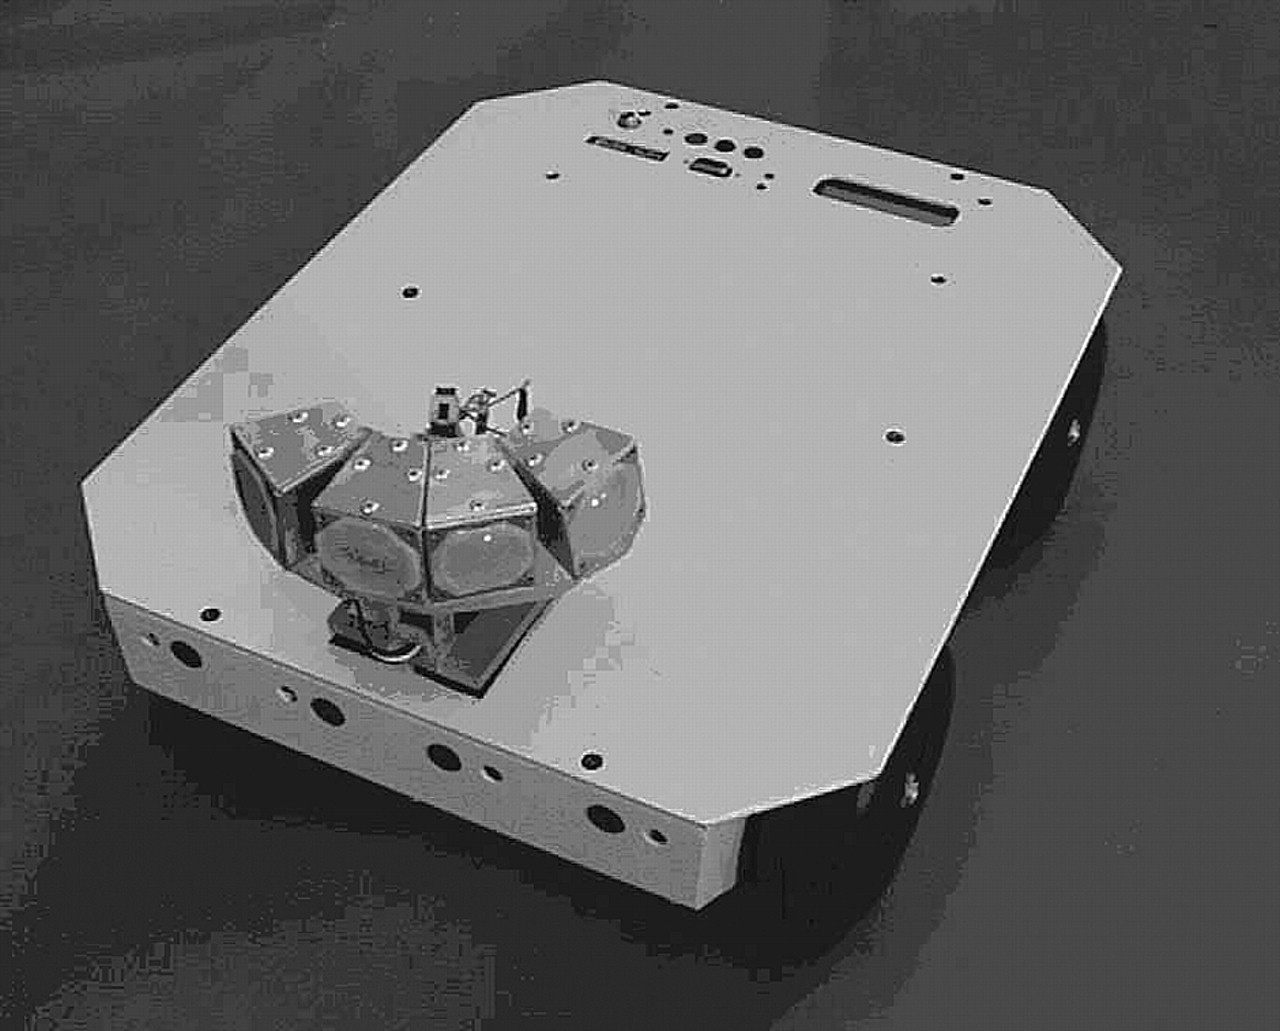
\includegraphics[width=4.5cm]{labo1}
		 \caption{Labo-1}
		 \label{fig:Labo1}
	\end{subfigure}
	\begin{subfigure}[b]{0.3\textwidth}
		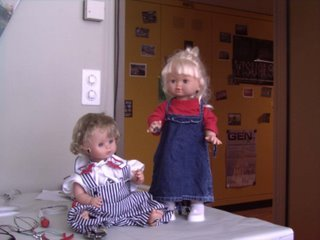
\includegraphics[width=4.8cm]{robota}
		 \caption{Robota}
		 \label{fig:Robota}
	\end{subfigure}
	\begin{subfigure}[b]{0.4\textwidth}
		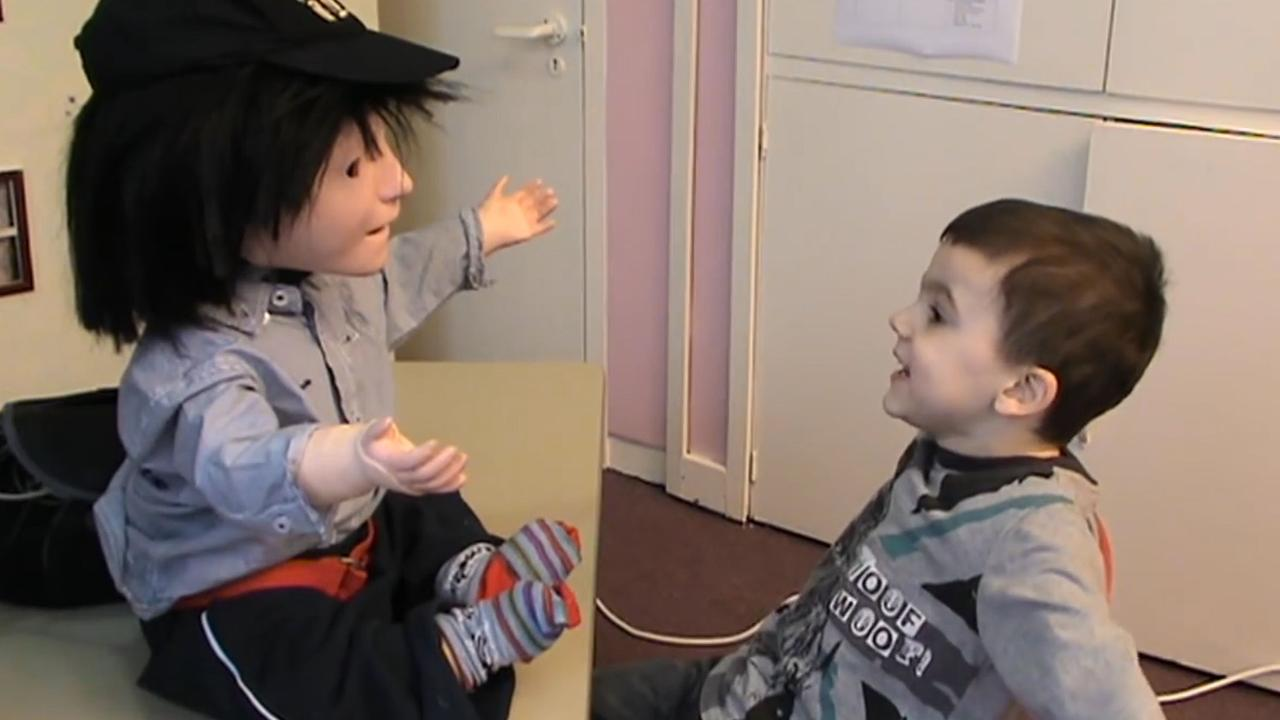
\includegraphics[width=6cm]{kaspar}
		 \caption{Kaspar}
		 \label{fig:Kaspar}
	\end{subfigure}
	\rule{35em}{0.5pt}
	\caption{Robots developed by Aurora Project}
	\label{fig:AuroraProjRobots}
\end{figure}

\subsection{Labo-1}
Labo-1 was the first robot developed by Aurora project\cite{werry1999applying}.It is a robust and \textit{mobile} flat-topped robot with 4 wheels, 8 infrared sensors, 1 heat sensor and, from the second version, 1 speech synthesizer. Thanks to its sensors, it is able to produce short spoken phrases using a neutral intonation and follow or escape from children avoiding obstacles. Its robustness and weight makes Labo-1 hard to pick up or damage from children. 
Trials done with four boys, aged between 8 and 12 years old, in order to improve \textbf{triadic interaction} and \textbf{turn-taking}.In a room with children, robot and therapist, the child was engaged in games that alternate the robot following turn to the go around turn. Children interacted with the robot without fear: some of them tried to clear obstacles from robot's path, one child smiled to the therapist for share his excitement and others tried to understand the robot's behavior observing its reactions to their continuous actions.
\subsection{Robota}
In 1998 the Aurora Project developed Robota\cite{billard1998experiments}, a doll-shaped humanoid robot. Its has motors that make arms, legs and eyes movable, it can speak thanks to his speech synthesizer, and can also understand lots key-words. Its camera processes the video, making Robota able to understand children movements and where they are looking to. When a children looks the robot, it starts to reply the movements performed by the children. This result as an improve in \textbf{imitation} and \textbf{eye-contact} behaviors. 
Robota was later\cite{billard2003robota} incorporated with a set of games focused on improve logic, coordination, and intellectual skills. This games are: dress the robot in the correct order, draw movements or positions in a PC or tablet that will be replayed by the robot, and interact(touching o performing movements) with the robot for answer to additions questions. Despite Robota seems to not intimidate children and during the studies were observed clear sign of enjoyment and social interaction, such as smiling and say goodbye, any case of spontaneous interaction occurred: it was always initiated by the teacher. Subsequent studies compared self-initiated interaction based on appearance, making trials with classic Robota and a plain version without eyes, hairs and plain dress. That study concludes that \textbf{children prefer to interact with a plain robot over a human-like robot}\cite{billard2007building}.

\subsection{Kaspar}
KASPAR is a minimally expressive \textbf{child-sized} humanoid robot designed for social interaction. In order to make it more attractive for ASD children, Kaspar has \textbf{simplified face} than an human(see appearance in \ref{designF}). It can show facial expressions, move his arms, hands, torso, head\cite{huijnen2016matching}, and speak using pre-recorded traces. It is used in \textbf{semi-autonomous manner}: the expert controls some Kaspar functionalities while other action are triggered from the robot sensors .
Children are encouraged in tactile exploration on Kaspar body and to repeat his facial expression, encouraging \textbf{eye-gaze} and increasing \textbf{emotion recognition} and body awareness with \textbf{turn-taking} \textbf{imitative} games. Another KASPAR’s purpose is to promote collaborative play with other children and adults, improving \textbf{triadic interaction}, and \textbf{joint attention}. 

The researchers conducted a study\cite{dautenhahn2009kaspar} in order to investigate how this robot could mediate the interaction between children with autism
and other people. During the interactions with KASPAR, children did not demonstrate aggressive behaviors towards the robot, they touched and gazed to its facial expressions in detail and also interacted with the present adult and social peers. So, it was possible to observe that KASPAR helped all the participants \textbf{to generalize their behavior} with the robot to others.

\section{Tito}
Tito\cite{duquette2008exploring} is a \textbf{mobile robot} with anthropomorphic shape. It has human stylized features such as movable arms, head and feet, despite it uses wheels for motion. Its face is composed by two eyes, a nose, and movable mouth. In one of the eyes, it has a camera able to measure eye gaze toward him. It uses pre-recorded messages for communication and it is controlled by wireless. Different parts of
Tito’s body can also be illuminated, and it is able to sense if it is being shaken or if it has flipped over.
\begin{figure}[h]
	\centering
	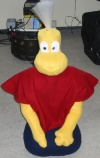
\includegraphics[width=0.4\textwidth]{tito}
	\caption{Tito}
	\label{fig:Keepon}
\end{figure}
Robots in general are more predictable and
less complex in their interacting modalities compared with a human and this robot has been created in order to analyze how effective are robots for ASD therapy compared with humans. A group of four children was split in two groups of two children each. The first group interacted with a robot mediator, the other one with a human mediator. In both cases children were engaged in three levels of imitation exercises: facial expressions, body movements, and familiar actions with or without objects. In both group, when the children imitated correctly, the mediator gave a sensory reward smiling, raising both its arms and saying 'Happy!'. The results showed that participants paired with Tito demonstrated more shared focused attention, visual contact, facial expression imitation and eye gaze directed toward the robot than ones paired with a human mediator. However, the children paired with the human mediator demonstrated, compared to the others, more evident increase on the imitation of words, gestures and body movements towards the other person in the room. 
In conclusion, the study showed that sensory properties of the robot (e.g. movements, colors, lights) managed to keep children interested in it but children paired with the human revealed higher results on imitation of body movements and of familiar actions. The authors hypothesized it was due to the restricted movement capabilities of the robot that did not allow children to understand their communicative intent.

\section{Keepon}
Hideki Kozima and his research group of Kyoto National Institute of Information and Communications Technology, developed interesting studies in the field of social robots for autism therapy\cite{kozima2009keepon}. Previously they built Infanoid, a upper-torso humanoid robot able to show facial expressions and other gestures. Researchers observed that the robot highly mechanistic appearance and its excessive expression of information caused attention dispersion and led to anxiety. Therefore, the researchers developed Keepon that, unlike Infanoid, has a minimal design that makes children feel more comfortable.
\begin{figure}[h]
	\centering
	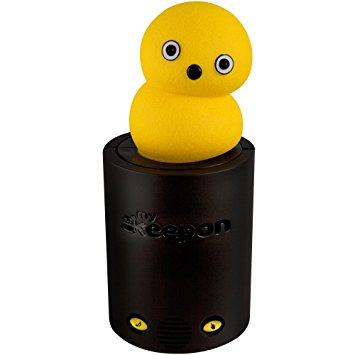
\includegraphics[width=0.4\textwidth]{keepon}
	\caption{Keepon}
	\label{fig:Keepon}
\end{figure}
Keepon is an anthropomorphic robot with a yellow snowman-like body, it is 12 cm tall and it is composed by tho parts: the head and the belly. The head has two eyes and a nose. Thanks to four DC motors, the silicon rubber material it is made, and small gimbals and wires installed in the belly, it is possible to manipulate Keepon's body, like a marionette.
Keepon can be autonomous or remote controlled, and it can orienting its face to a certain target and express its emotional states whenever the child makes any verbal or physical social interaction. It also interact coming up with rhythmic games, in form of structured music and dance sessions or with repetitive \textbf{turn-taking} and \textbf{imitation} behavior. Body movements are preprogrammed and it can exhibit excitement, pleasure and fear \textbf{emotions}, or simply dance.
Researches analyzed how the minimal design of Keepon could help children to understand social information and motivate them to share interests and feelings with others. Trials demonstrated that children spontaneously approached and started “tasting” Keepon's texture and motion, entering gradually into a complete social interaction with the robot. Thanks to simple and comprehensible ways used by the robot for exhibit its attention and emotions, children could understand the social meaning of the robot’s actions without becoming bored or overwhelmed. \textbf{Triadic interaction} and \textbf{joint attention} with peers and adult was also improved for some children: one children stops another while he was beating the robot; others shared joy or surprise to adults while they were interacting with the robot.
The research conclusion was that simple robots with  minimal and comprehensible expressiveness make easier understanding and extracting socially meaningful information for ASD children, encouraging so the expression of emotional states like surprise, pleasure or frustration.
\section{Paro}
PARO is an autonomous robotic seal equipped with sensors and actuators and computational intelligence that enables it to simulate the sounds and movements of a real baby harp seal. It has five kinds of sensors: tactile, light, audition, temperature, and posture sensors, with which it can perceive people and its environment. With the light sensor, PARO can recognize light and dark. He feels being stroked and beaten by tactile sensor, or being held by the posture sensor. PARO can also recognize the direction of voice and words such as its name, greetings, and praise with its audio sensor. It can also learn to behave in a way that the user prefers, changing the probability to do an action based on previous reaction(an hit or a pat) to that action. It can also responds to verbal question, moving its head, legs and making sounds. 
It is being used with great success in dementia care in Japan and Europe as a robot companion with the purpose of increasing quality of life and reduce stress and anxiety and to provide a therapeutic tool for specific individual interventions. Research suggests that PARO can be used as a facilitator of social communication for children with autism as well (Roberts \& Shore, 2013).
Researchers\cite{bertel2013peers} also conducted a three month case study on the use of PARO, at a school for children with autism, in order to study long-term interactions in real-world educational settings. The robot is used in order to motivate\textbf{ bodily or verbal attention}, involving children to touch it and to verbalize their thoughts; \textbf{create joint attention} with peers, asking children to touch the robot together touching eventually each other; \textbf{motivate social attention}, putting Paro in the center of a group of children and singing all together; and to \textbf{redirect attention}, asking children to help him in some activities.



\section{Nao \& Zeno}
Nao, developed by ,and Zeno, developed by, , are both \textbf{small-size humanoid} robots used for \textbf{imitative} and \textbf{turn taking} games. Therapy sessions are done with the robot placed on a table and the children sit on a chair in front of that. These robot can imitate children movements or engage them to imitate their movements, giving a positive sensory reward when the imitation is well done, or trying to motivate more or help the children if he is not able to imitate the movement. Zeno is used also to ask children to guess its mood. These robots are provided with a software for easy program the robot's behavior, and this makes them very customizable and this has permitted to use them for a lot of different studies. The setting of the interaction, unfortunately, results poor for autistic children: a therapist that controls the children does not touch the robot is needed, being the robot expensive and quite delicate. Another negative point are their rigid and jerky movements that furthermore need to be monitored because the robot can fall from the table. 
\section{Previous Teo}
Teo is an emotional, huggable, mobile and configurable robot developed by Politectico di Milano. Thanks to three omnidirectional wheels, its movement is holonomic, allowing it to freely move in any direction. Hidden on its body, Teo has a set of force sensing resistors that make it able to detect and distinguish hugs, caresses and punches. It is also equipped by a set of big mechanical buttons located on the head that can be personalized and permit children to express choices in response to different situation. A set of colored light, hidden in the body, are used to strengthen interaction and express emotions. An external depth sensor(kinect) can sense the motion of children making possible to display on a screen a virtual reality that encourages children to have a full-body interaction with the robot. 
Teo's cartoon-like with human simplified characteristics design stimulate ASD children to explore the interaction with it without any fear. One of the most important Teo's characteristic is personalization: sets of different mouths and eyes can be placed on the robot, creating a large number of different expression, or can be completely taken out, removing any human trait and making Teo more like an object than a person. Also mechanical buttons can be personalized, based on the ongoing activity or game, by colored tags or iconic images.
Teo can be remotely controlled, but it has also autonomous behaviors activated when sensors detect an interaction or during games.
\begin{figure}[h]
	\centering
	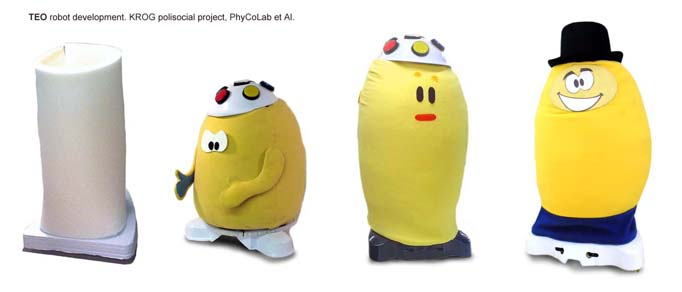
\includegraphics[width=0.9\textwidth]{prevTeo}
	\caption{Teo's shape history}
	\label{fig:prevTeo}
\end{figure}
Teo has been used in two exploratory studies. The first study involved 19 children aged between 6 and 12 years old that were split in two groups: one group, composed by children with most severe cognitive deficits, played alone, while children whose socialization problems were more severe than cognitive deficits, played with a peer. Three sessions were held weekly, the third was a group session, where children interact with Teo and all their classmates. Results highlights the importance to make more than one session with the robot: in both groups has been noticed an increase of positive behavior from the first session to the second. That increase, noticed in communication's skills, self-expression ability, attention loss frequency and interaction, was stronger in paired session, suggesting that group sessions are more effectively than alone ones. 
The second study involved 5 low functioning autistic subjects playing alone under a therapist's supervision for 10 weekly held sessions. In this study patients were engaged to answer to color-related questions made by Teo, touching the right button. A comparison between the number of right answers obtained 'with' and 'without' Teo emphasizes a wide difference, demonstrating the robot effectiveness.

% !TeX spellcheck = en_US
%*******************************************************************************
%****************************** Fourth Chapter *********************************
%*******************************************************************************
\chapter{System Design}
\label{chapter4}
% **************************** Define Graphics Path **************************
\ifpdf
\graphicspath{{Chapter4/Figs/Raster/}{Chapter4/Figs/PDF/}{Chapter4/Figs/}}
\else
\graphicspath{{Chapter4/Figs/Vector/}{Chapter4/Figs/}}
\fi

This new Teo(see...) has been developed for "Il Sogno" association, placed in Castelnuovo di Garfagnana, Lucca. It is inspired by previous Teo, keeping similar design and functionalities. Previous Teo was created in the context of 'Polisocial', hold in Politecnico di Milano and for this reason it is composed of multiple system developed by different groups of student. This gives a large number of different function to Teo, but it also makes difficult the phases of setup and control, requiring technician continuous intervention. The aim of this Teo is to create a robot with same features but easier to set up and with a user friendly control, in order to have a durable product with all-included-pieces and functionalities that can be easily used also by non-technician people. In this chapter will be firstly presented the \textbf{design choices} with reference to \ref{designF} and the \textbf{mobile Application} useful for navigate between Teo's modalities and \textbf{functionalities}, designed in order to improve in children different \textit{target behavior} useful for the treatment(see \ref{targetBe}).
\section{Design Features}\label{designFunct} 
Teo is an emotional, huggable and mobile robot characterized by soft body and a rigid base. Its \textbf{appearance} reminds characters of popular cartoons: it \textit{doesn't have relation with any real body} but it still has human characteristics like feet, eyes and mouth. It is about 90cm high, so its \textit{size} is comparable to children's one, resulting so visible and, at the same time, avoiding to generate fear due to its proportions. This simple and captivating shape, besides being less expensive and easier to implement than a human-shaped one, is able to be more attractive and to help interaction for children affected by ASD, allowing them to feeling familiar and safe.\\
Most robots developed so far interacts with children standing on a table at safe distance, avoiding that children touch, and possibly damage a robot that is usually quite expensive and delicate. Interaction with Teo, instead, is “free” and “full body”, this means that it can move in the space and it can be freely(randomly) caressed, cuddled or struck during the therapy sessions. There are 3 sonar sensors on the front of the base and one on the back. Thanks to them, Teo can detect if there is somebody or something in the environment and consequently define the movement direction. For reach its tactile features, the body is soft and equipped with a set of flexible capacitive sensors placed on the belly and on two areas of the back, one on the upper right and one on the upper left.\\
The soft body is fixed to the rigid base via 6 automatic buttons: 2 on front, 2 on each side and 2 on the back. The external yellow part, made with fleece, can be extracted and washed or replaced if it is necessary. Teo's face can be personalized: different eyes, mouth and eyebrows can be placed thanks to velcro strips in order to compose various moods and create strong emotional impact with children. This makes Teo \textbf{adaptable} to children needs:
a combination of patches or none can be applied based on individual children's reaction and feeling.
On the top of the head there are 4 capacitive buttons, that can be personalized in the same way of the face, and a luminous element. The buttons are used in order to navigate the basic menu and make choices during the exercises, meanwhile the luminous element allows to give an emotional feedback of robot’s status. On the back there is an useful pocket where patches of exercises and faces can be stored.\\
In order to reach \textbf{safety for both children and robot}, all hardware components(processor, sensors, motors and battery) are incorporated, and so hidden, in Teo's base. This avoids children to touch those components that they could damage or could injury them. Moreover, the base is designed to stay on the floor, not on a table, and this permits to Teo to freely move in the space without have fear that it falls from a table.
The base is the most “delicate” and important part of Teo, here are contained all hardware components so, in order to avoid damages, it is protected by a rigid thermoformed case. The robot is composed by a large number of \textbf{modular hardware components}, that can be easily replaced in case of troubles. On bottom right side of the thermoformed case, looking the robot from the front, there is a little hole that allows to reach the power button. Also this element has been hidden in a safe and protected place to avoid that users switch on or off the robot, without permission or intention. The battery, also included in the base, can be easily charged unplugging it from the system and plugging it to a battery charger. When battery is low and Teo is running, it informs about the lack of energy by verbal communication, if instead the robot is turned on with battery already under the minimum level, Teo informs about the state and it cannot be utilized until it is recharged.\\ 


\section{Android Application}
Teo is provided with an application for Android smartphones and/or tablets that permits to connect to the robot via bluetooth technology, allowing a complete, simple and speed control. The application is used for navigate between robot's modalities, change settings, trigger different actions, override robot's autonomous movements and collect data. 
Once the robot is turned on, it say 'Hello' and invites to choose between the two available modalities, that are:
\begin{itemize}
	\item Familiarization Modality
	\item Game Modality	
\end{itemize}
The functionalities available during this modalities is reported in the above sections.
	 

\iffalse
\subsubsection{Triskar}
that permits to the robot to move in holonomic way(its possible to control each degree of freedom) 
%\

The Swedish wheel functions as a normal wheel,
but it has little passive rollers around the
circumference.
-These rollers provide low resistance in another
direction.
-The wheels’ primary axis serves as the only actively
powered joint.

Swedish (Omni) Wheel:
-Three degrees of freedom;
rotation around the motorized
wheel axis, around the rollers,
and around the contact point.
-45 degrees or 90 degrees types.


- A robot is holonomic if the controllable degrees of
freedom are equal to the total degrees of freedom.
- If the robot is able to move in an arbitrary direction out of any
position at any time it is called holonomic.
- Consider a two-dimensional space; the degrees of freedom
are the x axis, y axis, and rotation about the origin. In this
space, a mobile base with three omnidirectional wheels in a
triangular configuration would be considered holonomic.
Stability of a vehicle is be guaranteed with 3 wheel
– center of gravity is within the triangle with is formed by
the ground contact point of the wheels.

Both Omni wheels and Mecanum wheels provide traction in normal wheel movement as any other wheel would. however, what makes these wheels special are the small rollers along the wheel's edges. These wheels are designed to provide a minimum amount of friction sideways allowing the wheels to move in any direction.

Omni wheels or poly wheels, similar to Mecanum wheels, are wheels with small discs around the circumference which are perpendicular to the turning direction. The effect is that the wheel can be driven with full force, but will also slide laterally with great ease. These wheels are often employed in holonomic drive systems.

The best choice for a robot that requires multidirectional movement. Omni wheels are normal wheels with passive wheels (rollers) attached
around the circumference of the center wheel.
Omni wheels can move in any direction and exhibits low resistance when they move in any direction. The small wheels are attached in such a
42way that the axis of the small wheels are perpendicular to the axis of the
bigger center wheel which makes the wheel to rotate even parallel to its own
axis.
\fi

\section{Familiarization Modality}
\label{FamMod}
Familiarization modality is designed for introduce the robot on first sessions and for free play. Sessions can be done involving a children, the robot and the therapist, improving \textbf{triadic interaction}. During this modality there are no limitations in children interaction: it is possible to engage children to different activities and the robot automatically reacts to determinate children actions. This feature results useful in order to improve \textbf{self-initiated interaction} and \textbf{cause-effect} of actions. After some trials, children can understand that based on their actions the robot reacts differently and this encourage them to maintain an interaction with it and to perform the right actions, with the aim to Teo acts as they want or like. Actions detected by the robot are:
\begin{itemize}
	\item loud noises (high volume), reacting differently if it is a very short sound or a long lasting sound. In case of prolonged noise, like scream or cry, Teo expresses fright and confusion making a backward snap. If the sound is short, like recall or whistle, it turns on itself and looks around. During the reactions, the LED emits a BLUE button light. 
	\item touches, that are classified based on intensity and the number of capacitives touched simultaneously. The types implemented are:
	\begin{itemize}
		\item \textbf{PAT}: In case of caress the robot vocally expresses happiness with a verse and the LED lights up with Blue. At the third caress received, expresses even more vocally happiness.
		\item \textbf{HUG}: In case of hug vocally expresses happiness and the led pulses with red color. A prolonged embrace starts a different audio that expresses further happiness. The embrace must touch at least 2 sensorized zones to be recognized.
		\item \textbf{HIT}: In case of a blow, the robot escapes, vocally expressing a sound of pain, and then approaching again but slowly. During the movement the LED turns orange. At the third consecutive shot the robot escapes and makes a movement of annoyance, warning not to beat him anymore. The lights pulsate Red.
	\end{itemize}
	
\end{itemize} 
During this modality, the application can used for trigger \textbf{both 'Direct Commands' and 'High-Level Controls'}. 'Direct Commands' are simple and single commands useful for control Teo's movement, play an audio, or change settings. This type of commands require the continuous intervention of the therapist but can result useful during the first sessions, when the child has to discover the robot, for personalize the interaction based on children's needs and what enjoy him. Direct Commands, available in Familiarization Modality are:
\begin{itemize}	
	\item \textbf{Change settings}: it is possible to turn on/off each sensor used to trigger robot's reactions to different actions(microphone, body capacitives), or make them more or less sensitive changing the threshold. It is also possible to change the pattern and color of  LEDs, switch them off and change the volume of speakers.
	
	
	\item \textbf{Robot's movement control:} the App simulates a remote controller useful for define movement direction and setting speed. Movement patterns can also be triggered. This kind of movements, that are pre-defined, help the therapist to trigger robot actions without to directly control it, and ensure that movement will be always the same, so children will became familiar to these and can learn to interpreter them.  
	
	\item \textbf{Play one of the available sounds}, that can be useful in order to start the interaction, saying phrases like "Hi!", "How are you?", or to entice child to have a therapist's monitored dialogue with the robot. Sentences that involve children to put an happy, sad or angry face on Teo can be useful for increase \textbf{emotional expression} capability.
	
\end{itemize}
High Level Controls \textbf{make the robot autonomous} or apply at the same time more 'Direct commads'. High Level Controls available in Familiarization Modality are:
\begin{itemize}
		\item \textbf{Trigger the robot's mood}. This states are expressed through lights, movements and phrases and can be more expressive with the right physical face applied on the robot. Children can be engaged to try to understand the robot's mood, helping to develop \textbf{emotion recognition}. After the movement is performed, speed and led color are fixed based on the triggered mood so, moving the robot, it still express that mood.
		The avaiable Teo's moods are:
		\begin{itemize}
			\item Happy
			\item Sad
			\item Angry
			\item Scared
		\end{itemize} 
		\item \textbf{Start or Stop the available Spatial Games, that are:}
		\begin{itemize}
			\item \textbf{Autonomous Movement}, which makes the robot go around the environment alone, avoiding obstacles and turning at random time.
			
			\item \textbf{Following Movement}, which allows the robot to follow the children keeping a minimum distance, avoiding to hit him. Using sonars, the robot moves in the direction of what it sees closer to itself until it reaches the set distance. It is possible that Teo make a mistake by approaching a wall due to sonars that cannot distinguish walls from people. In case the robot stops in front of a wall, thanks to the rear sensor it is possible to "wake him up" approaching his shoulders, making him notice that there is someone behind him. At this point Teo turns and start again with the chase.
			
			\item \textbf{Run Away/Chase Movement}, which mix the two previus movements. In this movement, the robot turns in the environment avoiding obstacles keeping body touch sensors active. If capacitors detect a touch, Teo stops and turns to the touch direction, assuming towards the children, and starts to follow him for 10 seconds, before return to free movement. The LEDs take on rainbow coloring. With the alternation of these behaviors, \textbf{turn-taking} and \textbf{self-initiated interaction} can be upgraded. 
		\end{itemize}
		during spatial games, direct \textit{Robot's movement control} commands can be used in order to \textbf{override the direction defined by the running algorithm}. This makes possible to 'deviate' robot's movement if it is not correct or if it is going too far from children.		
\end{itemize}

\section{Game Modality}
Game modality is used in order to improve \textbf{cognitive skills}, engaging the children in simple games where it is asked to touch the right figures after a robot's question. \textbf{Data collection} of number of right answer and time to answer are saved in the application, in order to evidence the improvements during the different sessions and so the effectiveness of the game. Once Game Modality has been selected, it is possible to choose the game and one of its different scenarios. Games differ each other for the type of questions are made, that should result easier in first game(Color) and harder in last one(Intruder Exclusion). In order to make the game more variable, each game has different scenarios that define which patches need to be attached on Teo, which question will be made and in which order. Once a scenario has been chosen, the application will show which patch must be attached on each Teo's capacitive. After all patches are applied, it is possible to start the game pressing a button in the application. Once game is started, the robot act completely autonomously. It makes questions and expect one or more answers, given touching the relative button. If a right question has done, Teo makes an happy movement, say "very good!" and its LEDs turn green; if instead the answer is wrong, the robot makes a movement similar to a 'no', says "wrong answer, try again!" and its LEDs turn red. At the end of both positive and negative movement Teo come back to its start position and, if the question is right and there are no further answers, makes a new question, if instead there are more answers or the answer is wrong, Teo will make again the same question. At the end of the game, based on the number of right answers that have been given at first attempt, Teo makes a different movement, an audio of congratulations and sends the data to the application.

\subsubsection{Color Game}
During Color Game, four colored buttons(red, yellow, blue, green) are applied on Teo's capacitive. The robot turns on its Leds with different colors and engage children to touch the button with same color.
\subsubsection{Color and Shape Game}
This game involves patch of different animals with different colors. Children are involved to touch patches of a declared color or to touch all those have the same color or the same animal. 
\subsubsection{Knowledge Game}
In this game children have to touch the patch asked from Teo that can make the request in a directly way, saying for example "Touch the chair", or with a indirect request, asking for example to "touch what you can eat" and expecting as answer 'ice cream' and 'sandwich'.
\subsubsection{Intruder Exclusion Game}
Harder question are made, involving animals, people, things and their categorization. Can be answered to touch "the animal that walks on two legs and doesn't fly", "the animal that flies", "the animal that runs" or to generically "touch the intruder".  
% !TeX spellcheck = en_US
%*******************************************************************************
%****************************** Fourth Chapter *********************************
%*******************************************************************************
\chapter{System Implementation}
\label{chapter5}
% **************************** Define Graphics Path **************************
\ifpdf
\graphicspath{{Chapter5/Figs/Raster/}{Chapter5/Figs/PDF/}{Chapter5/Figs/}}
\else
\graphicspath{{Chapter5/Figs/Vector/}{Chapter5/Figs/}}
\fi

\section{Hardware Setup}

Teo is a quite complex system composed by sets of controllers, serial devices, sensors and actuators. It is powered by a lead-acid battery that provide nominal 12V using six series-connected cells.
The hearth of the robot is the Arduino Mega, a microprocessor that analyze the flow of data coming from all the sensors in order to define what the actuators have to do. For this reason, each component of Teo is someway(directly or not) connected to Arduino Mega. Accelerometer and capacitive sensors are in charge to detect and classify touches, they are the only components that are not directly connected to Arduino Mega. In the starter project they should have been, but the way capacitives define their value, require excessive execution time, affecting the performance of overall the system. So we needed to add an extra controller, an Arduino Nano, that processes the data coming from the capacitives and the accelerometer, telling to the main processor where the robot has been touched and how.
In this section we will talk about general Teo's hardware architecture, giving a description of the controller and the list of serial devices, sensors and actuators that are included in the project and how they are connected each other. Details about each hardware component will be discussed in the next sessions, where each Teo's functionality will be analyzed.

\subsection{Arduino Mega}
Arduino is an open-source electronics prototyping platform, designed to make the process of using electronics in multidisciplinary projects more accessible\cite{arduino:intro}. 
It consists of a physical programmable circuit board with an Atmel AVR processor and on-board I/O support; and a piece of software, or IDE (Integrated Development Environment) that runs on a computer in order to write and upload the code.
Unlike most previous programmable circuit boards, the Arduino does not need a separate piece of hardware (called a programmer) in order to load new code onto the board, it can be done just using an USB cable.The Arduino IDE uses a simplified version of C++, making it easier to learn and program.\\
The project began in Ivrea, Italy in 2005 from Massimo Banzi and David Cuartielles.
The name Arduino comes from a bar in Ivrea, Italy, where some of the founders of the project used to meet. The bar was named after Arduin of Ivrea, who was the margrave of the March of Ivrea and King of Italy from 1002 to 1014\cite{lahart2014taking}.\\
There are several Arduino boards, that differs for number of analog and digital I/O pins, processor and memory.
In this project we used an Arduino Mega as controller of the overall system. It has 54 digital input/output pins (of which 15 can be used as PWM outputs and 6 can be used to attach interrupts), 16 analog inputs, 4 UARTs (hardware serial ports), a 16 MHz crystal oscillator, a USB connection, a power jack, an ICSP header, and a reset button\cite{arduino:mega}.\\
As shown in \ref{megaConnections}, each component of the system, except to capacitive sensors and accelerometer, is connected to the Arduino Mega that, based on the senors values(inputs) and the robot state, defines what the actuators(outputs) have to do.
\begin{figure}[h]
	\centering
	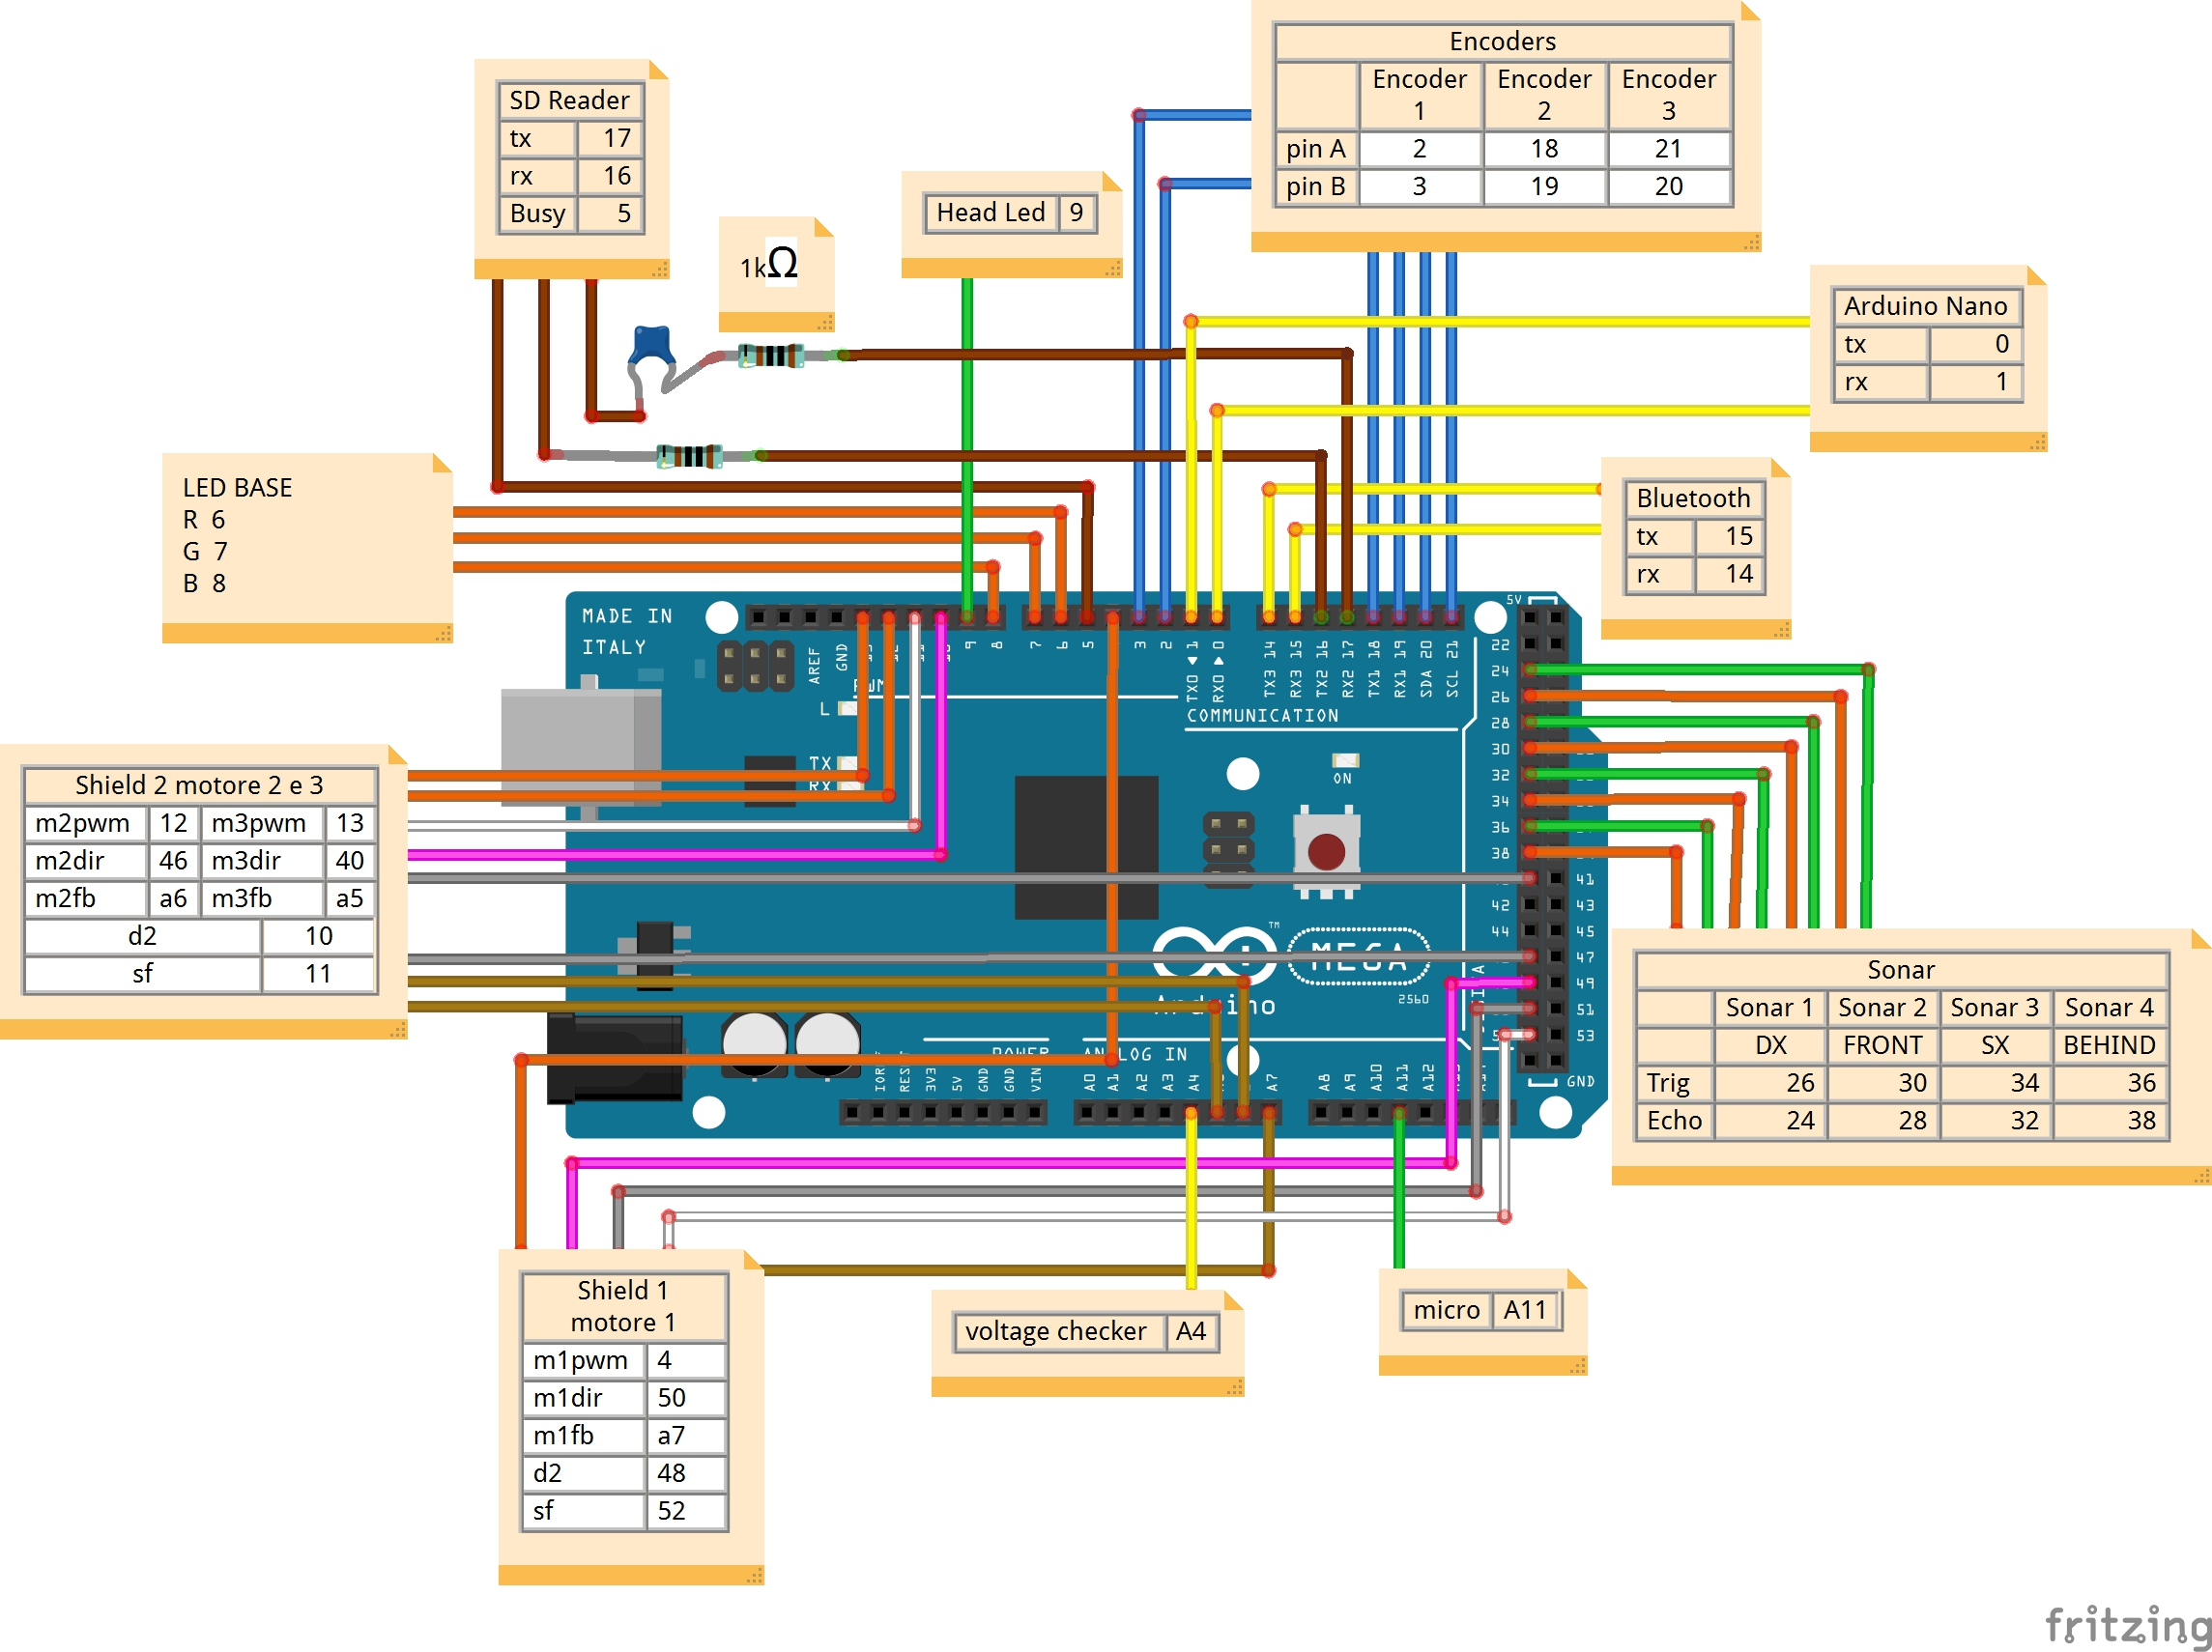
\includegraphics[width=1\textwidth]{TeoG2_bb}
	\caption{Arduino Mega connections}
	\label{megaConnections}
\end{figure}
\subsection{Serial Devices}
Arduino Mega has four UART(Universal Asynchronous Receiver/Transmitter) ports. Unlike Parallel interfaces that needs a lot of wires to transmit data, serial interfaces stream the data, sending one single bit per clock, so these interfaces can operate using only two wires: one receiver(RX), and one transmitter(TX). For this propose, Arduino Mega has eight dedicated pins.
In this project we used three Serial ports, so six pins, in the following table are listed the utilized ports, and for each one the RX and TX pin, and which device is connected to.
\begin{table}[h]
	\centering
	\begin{tabular}{|l|l|l|l|}
		\hline
		\multicolumn{1}{|c|}{\multirow{2}{*}{\textbf{\begin{tabular}[c]{@{}c@{}}Serial\\ Number\end{tabular}}}} & \multicolumn{2}{c|}{\textbf{Pin}} & \multicolumn{1}{c|}{\multirow{2}{*}{\textbf{\begin{tabular}[c]{@{}c@{}}Connected\\ Device\end{tabular}}}} \\ \cline{2-3}
		\multicolumn{1}{|c|}{} & \textbf{TX} & \textbf{RX} & \multicolumn{1}{c|}{} \\ \hline \hline
		Serial 0 & 1 & 0 & Arduino Nano \\ \hline
		Serial 2 & 16 & 17 & DF Player \\ \hline
		Serial 3 & 14 & 15 & HC-05 Bluetooth Module \\ \hline
	\end{tabular}
	\caption{Serials connections}
	\label{tab:Serials}
\end{table}\\
Looking the table its immediately evident that Serial 1 has not been included. that's because it is accessible by pin 18 and 19 that have, besides to 'serial' communication, dedicated hardware also for manage interrupts, which are necessary to guarantee an adequate functioning of the encoders. In sect.\ref{encoder} will be better discussed why interrupts are useful for the encoders.
So we were forced to use Serial 0 for the communication with Arduino Nano. Serial 0, on pin 0 and 1, uses the same UART port used by USB connection during a software update and, if both are connected, there's an obvious interference that makes mandatory to physically disconnect the serial port wires and restart Arduino. In addition to the possibility that this is rather boring, it can also cause breakdowns or loss of time when forget to disconnect the cables. But it was the last serial port available, so our choice was mandatory.
\\\\





\subsection{Sensors}
%\subsection{HC-SR04}
Teo is equipped by a lot of sensors:
\begin{itemize}
	\item four ultrasonic ranging modules(HC-SR04)
	\item one microphone sensor(Sunfounder Sound Sensor)
	\item seven capacitive sensors
	\item one accelerometer(MPU6050)
	\item three 30:1 Metal Gearmotor 37Dx68L mm with 64 CPR Encoder
	\item one battery level checker
\end{itemize}







\subsection{Actuators}
To make interaction possible and attractive, Teo has been equipped by different actuators:
\begin{itemize}
	\item two Pololu Dual MC33926 Motor Driver Shield for Arduino
	\item two speakers connected to the DFPlayer(see \ref{DFPlayer})
	\item one non addressable RGB LED strip
	\item one addressable Adafruit NeoPixel RGB Led Strip
\end{itemize}
\section{Bluetooth Connection}
Using Bluetooth Connection, a tablet or a smartphone that run Teo's application can be connected to the robot in order to send instruction and receive data. To make the connection, a blueooth module has been connected to the Arduino Mega(see \ref{tab:Serials}) and different states have been created in order to manage the instructions received and the data to send during the robot's different phases of use. 

\subsection{Bluetooth Module(HC-05)}
HC-05 is one of the most popular and cheapest module used for RF communications. It has ten meters range and allows to transform the Serial port of the Arduino Mega in a Bluetooth port, generally with a SPP(Serial Port Profile), thus becoming a serial over Bluetooth. 

\begin{figure}[h]
	\centering
	\begin{subfigure}[b]{0.4\textwidth}
		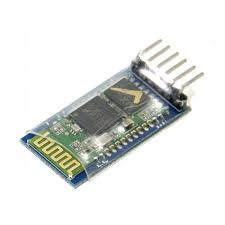
\includegraphics[width=4cm]{hc05-1}
	\end{subfigure}
	\begin{subfigure}[b]{0.4\textwidth}
		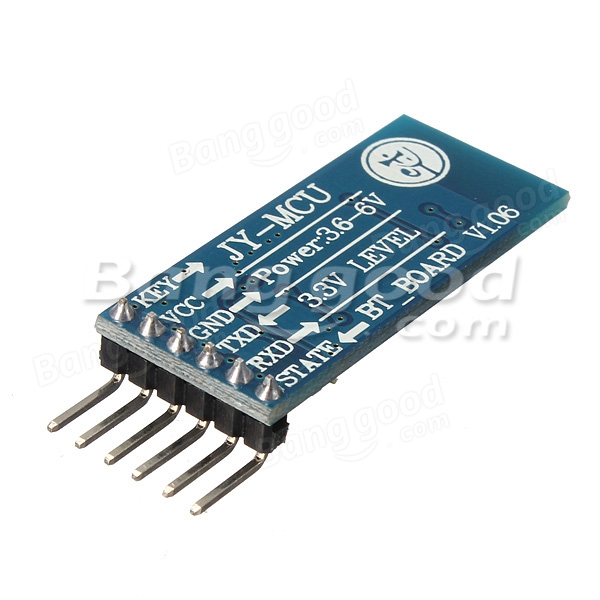
\includegraphics[width=4cm]{hc05-2}
	\end{subfigure}
	\rule{35em}{0.5pt}
	\caption{HC-05 Bluetooth Module}
	\label{HC-05}
\end{figure}
As show in \ref{HC-05}, the module has six pins, but we used only four of them: two for the power,VCC and GND connected respectively to Arduino's 5V and GND pins, and two for the serial communication(see fig.\ref{megaConnections}).
In order to work, it's important to keep in mind that the RX pin of the Arduino must be connected to the TX pin of the Bluetooth module, and, in the same way, the TX pin of the Arduino must be connected to Bluetooth RX pin.
The module can be easily set up with AT commands defining name, password, bound rate, modality(slave or master) and more.
In tab.\ref{ATCommands} it's possible to have a look on main HC-05 AT commands.
In this project, it is set with a 38400 baud rate and slave modality: the master will be the phone or tablet that will connects to it.
\\
\begin{table}[]
	\centering
	\begin{tabular}{|l|l|}
		\hline
		\textbf{Command} & \textbf{Description} \\
		\hline
		\hline
		AT & AT interface connection test \\
		\hline
		AT+RESET & Component restart \\
		\hline
		AT+ORGL & Restore to default settings \\
		\hline
		AT+ADDR? & Get module address \\
		\hline
		AT+NAME? & Get module name \\
		AT+NAME=<param> & Set module name equal to "param" \\
		\hline
		AT+ROLE? & Get module role(0=Slave/1=Master) \\
		AT+ROLE=<param> & Set module role to "param"(0=Slave/1=Master) \\
		\hline
		AT+PSWD? & Get PIN code \\
		AT+PSWD=<param> & Set PIN code equal to "param" \\
		\hline
		AT+UART? & Get Serial parameters \\
		AT+UART=<param1>,<param2>,<param3> & Set Serial parameters \\
		& (param1: Baud, param2: Stop bit, param3: Parity)\\
		\hline
	\end{tabular}
	\caption{AT Commands List}
	\label{ATCommands}
\end{table}
\subsection{Communication states}
The application presents different pages with different commands, based on the selected modality. Each page available in the App has a corresponding state on Arduino. In order to navigate between the different pages, once a choice has been made, the application sends via serial port a character that is interpreted by Arduino and define the new state and, consequently, the new page. 
Blueooth states are:
\begin{itemize}
	\item \textbf{chooseModality}: this is the initial state. It waits that the user choose between Familiarization Modality and Game Modality.
	\item \textbf{chooseGame}: once Game Modality has been chosen, this state is activated. This waits that the user choose which game will be performed.
	\item \textbf{chooseScenarioFamMod}: once a game has been chosen, one of the available scenario must be selected. This state waits that selection.
	\item \textbf{sgWaiting}: After the selection of the scenario, the application shows which patches put on which capacitive and invites to press a start button when the positioning is done. This state wait that the start button is touched.
	\item \textbf{gameModality}: when game is definitively started, the robot will act autonosmly so no one command will be send from the application until the end of the game. This state is active during all game session and when game finish it sends game data and  automatically turn to chooseModality state.
	\item \textbf{famModality}: if during chooseModality state 'Familiarization Modality' is chosen, famModality state is activated. During this state it is possible sends a lot of commands to Arduino(see \ref{FamMod}) and it also sends sensors data, with the aim to inform if sensors are working correctly.
	\item \textbf{discharge}: If battery is discharged when Teo is started up, the bluetooth state switch to discharge. In this state is impossible to give any instruction to the robot that must be charged.
\end{itemize}



\section{Basic Robot's movement control}
One important characteristic of Teo is the ability to freely move in the environment. As many others robots developed in AIRlab, Teo can move using Triskar base. It is composed by a set of 3 omni-directional wheels, each one driven by an independent gearmotor and equipped by an encoder. Two motor shield are used for control direction and power of gearmotors. This set of hardware, with an appropriate interpretation of data by software, permits to have a controlled movement of the robot, defining speed, direction and knowing at each moment where the robot is respect to its initial position. This makes also possible to create movement patterns that the robot can perform autonomously.
\subsection{Triskar base}
Triskar base is an hexagonal metal plate with 15cm of radio. Three wheels of 7cm diameter with connections at L of 4 cm length are fixed at 3 sides of the hexagon so, at \ang{120} of distance each other.
A three wheel design offers greater traction as any reactive force is distributed through only three points and the robot is well balanced even on uneven terrain. This design also reduces an additional wheel compared to a 4 wheeled robot which makes it cost effective (omni
wheels are expensive). Omnidirectional wheels, better explained in the above section, make Teo able to have an Holonomic Drive: it means that the robot has three controllable degrees of freedom and so, can always translate, rotate or both in any direction, avoiding to do any maneuver.
\subsubsection{Omnidirectional Wheels}
Omnidirectional wheels have passive rollers attached around the circumference of the center wheel which are perpendicular to the turning direction. The effect is that the robot can move in any direction and wheels  exhibit low resistance also when the movement is perpendicular to the wheel, because it can slide laterally with great ease.
\begin{figure}[h]
	\centering
	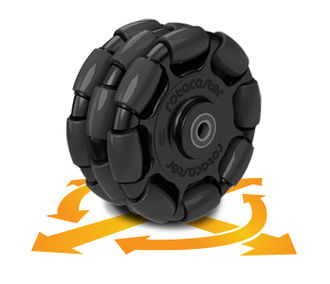
\includegraphics[width=0.3\textwidth]{omniwheel}
	\caption{Omni-directional Wheel}
	\label{fig:omniWheel}
\end{figure}
\subsubsection{Gearmotor with Encoder}
\label{encoder}
This gearmotor is a powerful 12V brushed DC motor with a 30:1 metal gearbox and an integrated quadrature encoder that provides a resolution of 64 counts per revolution of the motor shaft, which corresponds to 1920 counts per revolution of the gearbox’s output shaft. These units have a 0.61"-long, 6 mm-diameter D-shaped output shaft\cite{encoders}.\\
\begin{figure}[h]
	\centering
	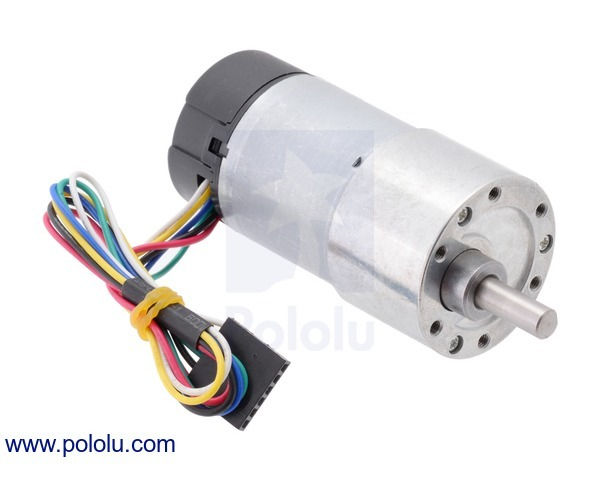
\includegraphics[width=0.5\textwidth]{gearmotor}
	\caption{Metal Gearmotor 37Dx68L mm 30:1 with 64 CPR Encoder}
	\label{fig:gearmotor}
\end{figure}
Incremental rotary encoders are widely used due to their low cost and the ability to provide signals about how much turns the gearmotor has done that can be easily interpreted and used to calculate a lot of data about Teo movement like position, orientation, speed of each wheel and of the entire robot. These data are reliable only in the presence of a floor that guarantees pure rolling motion($v=0$, $\omega\neq0$) to the wheel avoiding tangent slips and this, unfortunately, is only ideal and in reality means a loss of precision in function on the adhesion coefficient of the floor. Teo will work in indoor where it's hard to find and impervious or irregular floor and being a social robot, his movement doesn't have to be strictly precise. For this reason these encoders results as a good choice for have a feedback about Teo's movements.\\In order to work, quadrature encoders contain a code disk that is composed by two tracks, usually denoted as Channel A and Channel B. These tracks or channels are coded ninety electrical degrees out of phase, as indicated in the image \ref{fig:quad_enc_phase}, and this is the key design element that will provide the quadrature encoder its functionality.
\begin{figure}[h]
	\centering
	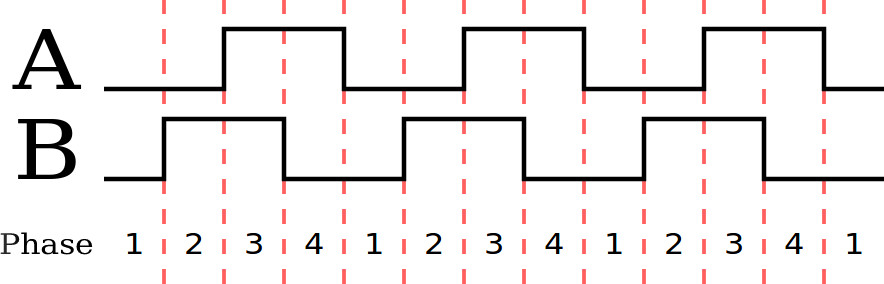
\includegraphics[width=0.8\textwidth]{encoder}
	\caption{Square waves in quadrature (clockwise rotation).}
	\label{fig:quad_enc_phase}
\end{figure}
\\
As illustrated in the fig.\ref{fig:quad_enc_phase}, when the quadrature encoder is rotating in a clockwise direction its signal will show Channel A reach the value of Channel B with one phase delay, and the reverse will happen when the quadrature encoder rotates counterclockwise.

Knowing direction, also position can be monitored. Each time one of the two channels changes its value, a counter EncCounter is incremented(clockwise rotation) or decremented(counterclockwise) based on the direction. The encoder mounted on our motor, has 1920 counts per revolution so, we can map the counter EncCounter to a degree position value and, knowing the radio R of the wheel(equals to 16cm), to a linear position value.
$$radPos= \frac{EncCounter\times2\pi}{1920}$$
$$linearPos= radPos\times R$$
Knowing the position of each wheel, speed can be derived and using inverse kinematic, is possible to define which is the real movement of the robot(look PID chapter).\\

Each gearmotor has six pins, 2 connected to the 12V battery positive and negative terminals, 2 inputs connected to Pololu Dual MC33926 Motor Driver Shield from which comes the commands  that allow motor to turn, and 2 encoder outputs(channels A and B)  connected to Arduino Mega external interrupt pins. Arduino Mega has six pins(2,3,18,19,20,21) that are able to attach interrupts and that is exactly the number of pins needed with three encoders. These pins can be set to trigger a function when the input signal is RISING or FALLING. The triggers are interpreted by hardware, so the interrupt is very fast. 
This project is full of devices that needs to work always in parallel and, being interrupts able to making things happen automatically and with maximum priority when it is needed, use them for the encoders is useful to insure that a pulse will never be missed, allowing Arduino Mega keep to manage also the other components.

\subsubsection{Pololu Dual MC33926 Motor Driver Shield}
This motor driver shield make it easy to control two bidirectional, brushed DC motors. Teo has two of them, in order to control its three wheels. As can be seen in fig.\ref{fig:dualmcscheme}, it is composed by two side, the logic one, connected to Arduino Mega, and the motor one, connected to gear motors.
\begin{figure}[h]
	\centering
	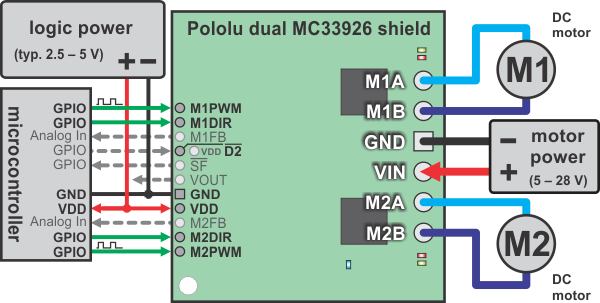
\includegraphics[width=0.6\textwidth]{dualmc21}
	\caption{Motor Driver Shield Scheme}
	\label{fig:dualmcscheme}
\end{figure}
On logic side there are VCC and GND pins for 5V power, D2 pin used to enable or disable motor driver outputs, and one PWM and DIR pin for each motor M1 and M2. The PWM pin define the power and DIR the direction of the motor. It's important to connect PWM pins on one of the fifteen Arduino PWM pins.\\
Pulse Width Modulation, or PWM, is a technique for getting analog results with digital means. Digital control is used to create a signal switched between on and off. This on-off pattern can simulate voltages between 5 and 0 Volts by changing the portion of the time the signal spends on versus the time that the signal spends off. The duration of "on time" is called the pulse width. Modifying the pulse width different analog values are obtained.\\
On motor side there are VIN and GND pins for 12V power and two pins that, based on PWM and DIR values on logic level, give the right voltage to gearmotors making them turn.
\subsection{PID}
\subsection{Inverse Kinematic}
\subsection{Direct Kinematic}
\subsection{Odometry}
\subsection{Movement Patterns}
\section{Sonars Management}
\subsection{Ultrasonic Ranging Modules(HC-SR04)}
To maintain a safer distance from the obstacles, three ultrasonic sensors are implemented on the front side and one on the back. HC-SR04 provides stable and accurate distance measurements from 2 to 400cm, with a focus of 15 degrees and a ranging accuracy that can reach up to 2mm.

Like bats and dolphins do, this sensor measures distance using ultrasonic sound that has such a high pitch that humans cannot hear. This particular sensor sends out an ultrasonic sound that has a frequency of about 40 kHz.\cite{hcsr04:datasheet}

\begin{figure}[h]
	\centering
	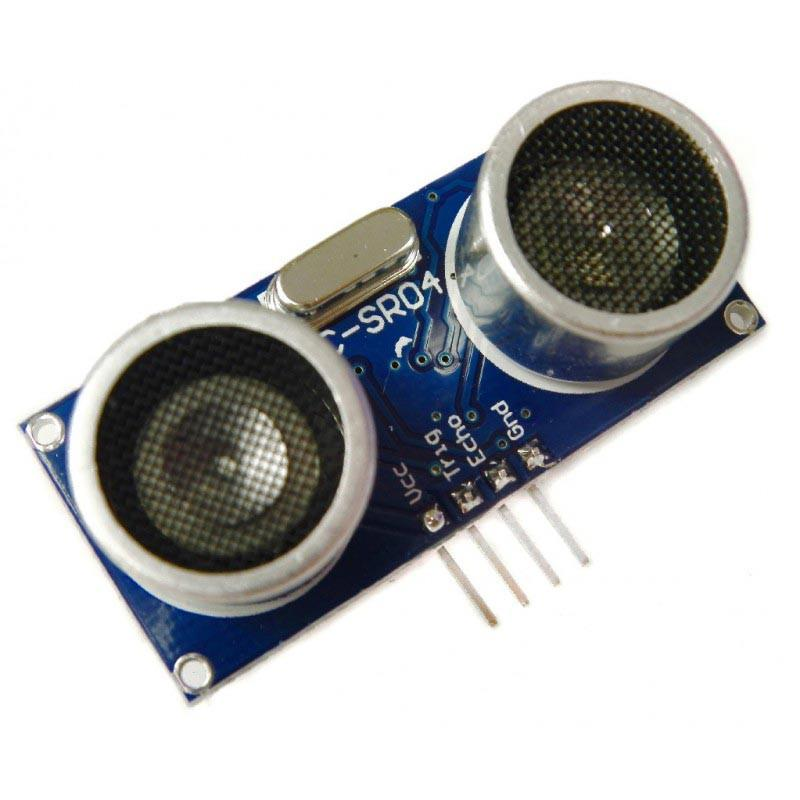
\includegraphics[width=0.3\textwidth]{hc-sr04}
	\caption{HC-SR04 module}
\end{figure}

The module is composed by an ultrasonic transmitter, a receiver and a control circuit. The transmitting phase of the sensor is called PING and it will wait for reflected signal from any obstacle in its path. This reflected signal is called ECHO. Taking trace on the time between when ping is sent and echo is received by the controller, it's possible to define the distance, using the following formula:

$$Distance = \frac{(Time \times SoundSpeed)}{2} $$

Sound travels at approximately 340 meters per second that corresponds to about 29.412µs per centimeter. The distance obtained multiplying $time\times speed$ must be divided by 2 because the signal sent from the sensor have to travel until it bounces on a surface and then return back, making the same distance two times.\\
The module has four pins: two(VCC and GND) for the power, and two(Echo and Trigger) used in order to communicate with Arduino.

DIGRESSIONE SU COME SONO MESSI I SONAR(ANGOLO DI VISUALE CON DISEGNO DEI CONI DEI TRE SONAR AFFIANCATI E IMMAGINE DEI SONAR DI TEO)
\subsection{Sonars orientation}
As you can see in picture NN, the 3 sonars on the front are oriented in order to have a 90 degrees vision. This allows Teo to have a reasonable view of the obstacles present in the environment, making it consequently able to autonomously navigate in the space.
\subsection{Input filtering and classification}
\section{Audio Playback}
\subsection{DF Player}
\label{DFPlayer}
The DFPlayer Mini MP3 Player for Arduino is a small and cheap MP3 module with an simplified output directly to the speaker. The DFPlayer perfectly integrates hard decoding module, which supports common audio formats such as MP3, WAV and WMA including 30 level adjustable volume and 6 level EQ adjustable. Besides, it also supports TF and MicroSD card with FAT16 or FAT32 file system. Thanks to this module is possible, through a simple serial port, to play any audio file, without great effort.

\begin{figure}[h]
	\centering
	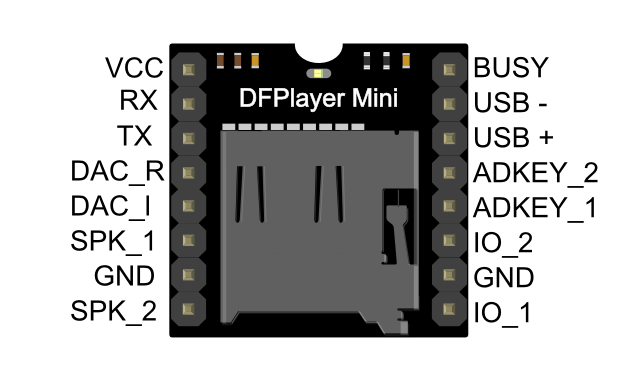
\includegraphics[width=0.6\textwidth]{dfplayer}
	\caption{DFPlayer module}
	\label{fig:DFPlayer}
\end{figure}
\subsection{Speakers}
As already talked in sec.\ref{DFPlayer}, Teo has two speakers that make it able to speak, play music and make various sounds. These are connected to the DF Player SPK\textunderscore1, SPK\textunderscore2 and ground(GND) and positioned on the bottom side of Teo, where they can be well listen but can't be reached and touched by children, avoiding they to damage them.
\subsection{Software Management}
\section{Touch Detecting}
\subsection{Arduino Nano}
The Arduino Nano is a small and complete board based on the ATmega328. It has 22 digital input/output pins (of which 6 can be used as PWM outputs), 8 analog inputs, one UART (hardware serial ports), and works with a Mini-B USB cable instead of a standard one\cite{arduino:nano}.\\
In this project the Arduino Nano is a bridge between the Arduino Mega and all the sensors(capacitives and accelerometer) that deal with detecting and classifying touches.
\begin{figure}[h]
	\centering
	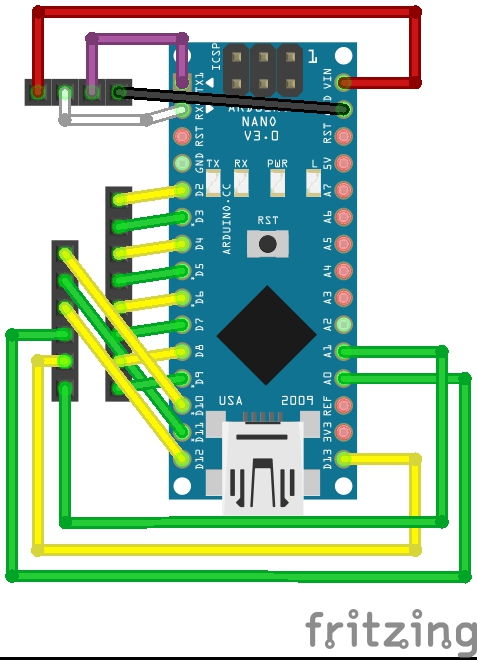
\includegraphics[width=0.4\textwidth]{arduinoMicroSchema_bb}
	\caption{Arduino Nano connections}
	\label{nanoConnections}
\end{figure}

\subsection{Communication between two Arduinos}
\subsection{Capacitive Sensors}
\begin{figure}[h]
	\centering
	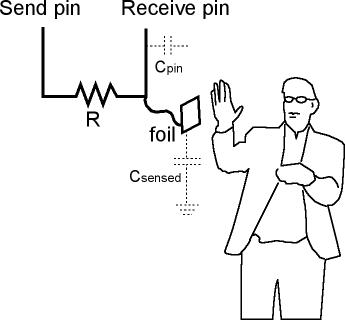
\includegraphics[width=0.3\textwidth]{CapSense}
	\caption{How Capacitive sensors work}
\end{figure}
Capacitive senors are a very important and innovative element for Teo functionalities.\\
There are seven capacitive sensors on Teo: three on the body(one on the belly, two on the back), used to detect touches and classify them in pats, hits and hugs, and four on the head, used in Game Mode in order to answer questions. 
The sensors have been completely developed by us with easy to find and cheap material, so the cost is very low. We had to try a lot of different configuration(see REF) in order to have good results. 

The setup includes an high value resistor(10MOhm) between the send pin and the receive (sensor) pin. The receive pin is the sensor terminal that, connected to a metallic net, makes the capacitive area.

When the send pin changes state, it will eventually change the state of the receive pin. The delay between the send pin changing and the receive pin changing is determined by an RC time constant, defined by $R \times C$, where R is the value of the resistor and C is the capacitance at the receive pin, plus any other capacitance (e.g. human body interaction) present at the sensor(receive) pin\cite{CapSenseLib}. Being $R$ a constant, bigger will be the capacitance means a big delay.\\

Being Teo powered by a battery, arise a ground problem for capacitors. 
-SPIEGARE MEGLIO-
attaccati al pc abbiamo un riferimento di massa invariato nel tempo, essendo la massa connessa a terra
con la batteria il riferimento di massa è variabile nel tempo, non essendo più costante, si perde stabilità ed efficienza.

mettendo la massa dietro, quando una persona tocca, la viariazione di capacità aumenta, e la massa relativa della batteria viene influenzata dalla mesa a terra del soggetto che tocca

The solution was to put another metallic net, connected by a wire to the battery ground pin, under the sensor net, insulated by a synthetic polyester wadding((FIBRA DI POLIESTERE(ovatta sintetica in poliestere)).Che isola lasciando flessibile e lasciando la possibilità di premere e deformare. This worked really well to stabilize sensor values and also seemed to efficaciously increase sensor sensitivity.

PARLARE DEL PROBLEMA DI OCCUPAZIONE DEL PROCESSORE PER TEMPO INDETERMINATO CHE HA SPINTO AD USARE UN ARDUINO EXTRA


\subsection{Accelerometer(MPU6050)}

\begin{figure}[h]
	\centering
	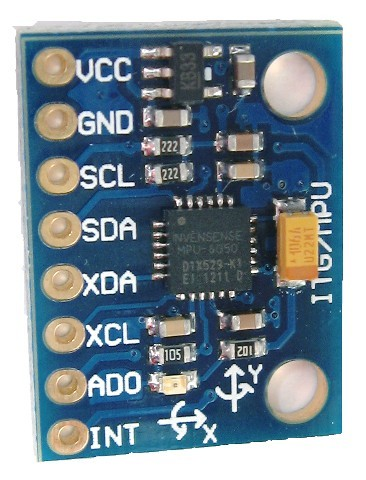
\includegraphics[width=0.2\textwidth]{mpu6050}
	\caption{MPU-6050 module}
\end{figure}


Able to capture the acceleration on the three axes, used with the capacitive sensors to define when the robot is hitten.

The MPU-6050 sensor contains a MEMS accelerometer and a MEMS gyro in a single chip. It is very accurate, as it contains three 16-bits analog to digital conversion hardware for digitizing the gyroscope outputs
and three 16-bit ADCs for the accelerometer outputs. Therefor it captures the x, y, and z channel at the same time. The sensor uses the I2C-bus to interface with the Arduino.\cite{MPU6050}

The MPU-6050 is not expensive, especially given the fact that it combines both an accelerometer and a gyro.
\subsection{Touch classification}
\subsection{Touch reactions}
\section{Micro Detecting}
\subsection{Microphone Sensor(Sunfounder Sound Sensor)}
\begin{figure}[h]
	\centering
	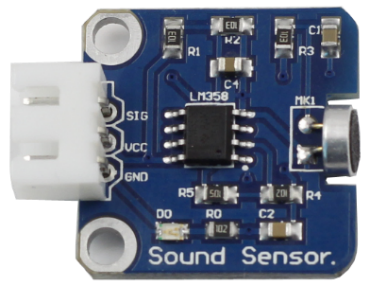
\includegraphics[width=0.3\textwidth]{soundSensor}
	\caption{Sunfounder Sound Sensor}
\end{figure}
Sound sensor is a component that receives sound waves and converts them into electrical signal. It detects the sound intensity in ambient environment converting audio signals into electrical signals. This module is used for detect high audio noise around the robot, such as screams. It has 3 pins, 2 for the power(5v), and one is the signal sensor output, connected to A11 Arduino analog-in pin. 
\subsection{Filtering and threshold}
\subsection{Reaction Behaviors}

\section{Leds Management}
\subsection{Non Addressable RGB LED Strip}
\label{LEDSTRIP}
A multicolor non addressable RGB LED strip is positioned on the bottom of Teo, just around the chassis. An RGB element is composed by three different LEDs(red, green, blue) arranged so can interact each other to form different complementary colors. Non addressable means that all strip LEDs display the same color at any time and this can be manipulated varying the voltage applied to each of the three power inputs, connected trough a MOSFET to Arduino Mega's PWM pins.


\subsection{Adafruit NeoPixel Addressable RGB LED Strip}
An Adafruit Multicolor Addressable RGB LED Strip has been placed on the head of Teo. In this LED strip, unlike the one of previous section(Sect.\ref{LEDSTRIP}),is powered by 5V and each LED has its own chip and can be individually triggered for color changing. Thanks to this, LEDs in the strip can light up in different colors at the same time \cite{schiller2010automated}.
Thanks to Adafruit library, this strip also needs an easier setup compared to the previous one, it has only one input pin directly connected to a PWM Arduino's pin and two pins for 5V power.
\subsection{Led Patterns and colors}

\section{Autonomous Movements}
\subsection{Exploring}
\subsection{Following}
\subsection{Mixed Movement}
\section{Moods Expression}
\subsection{Happy}
\subsection{Sad}
\subsection{Scared}
\subsection{Angry}

\section{Game Alghorithm}
\subsection{Data Collection}
\section{Battery Level Check}
Arduino analog inputs can be used to measure DC voltage between 0 and 5V. Teo's battery provides nominal 12V, it means it's voltage will be between 11.5V when discharged and 13.5V when fully charged. In order to measure voltages greater than 5V, two resistors have been used to create a voltage divider able to proportionally decreases the battery voltage to one within the range of the Arduino analog inputs. 

\begin{figure}[h]
	\centering
	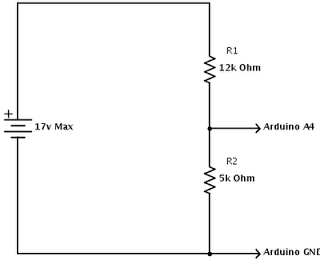
\includegraphics[width=0.5\textwidth]{voltage-divider}
	\caption{Voltage Divider Diagram}
	\label{fig:voltageDiv}
\end{figure}

With the aim to protect Arduino pins from voltages higher than 5V, we assumed an overestimated the maximum value of the battery, 17V instead of 13.5V, that is the usual voltage value of a full charged battery, and applying the voltage divider formula with the selected resistances $R1=\SI{12}{\kohm}$ and $R2=\SI{5}{\kohm}$
$$V_{out}=V_{in}\frac{R2}{R1+R2}=17V\frac{\SI{5}{\kohm}}{\SI{5}{\kohm}+\SI{12}{\kohm}}=5V$$
we can see that with $V_{in}=17V$ the voltage on Arduino Mega($V_{out}$) will be 5V. Being $V_{in}=17V$ a maximum overestimated value, we can ensure that $V_{out}$ will never exceed 5V.
The code in the Arduino Mega is in charge to recalculate the battery voltage value starting from the voltage received on the analog pin and, in case it is lower than 11.5V, Teo will warn the therapist about its need to be charged. 
%*******************************************************************************
%****************************** Sixth Chapter *********************************
%*******************************************************************************
\chapter{Experiments and Results}
\label{chapter6}
% **************************** Define Graphics Path **************************
\ifpdf
\graphicspath{{Chapter6/Figs/Raster/}{Chapter6/Figs/PDF/}{Chapter6/Figs/}}
\else
\graphicspath{{Chapter6/Figs/Vector/}{Chapter6/Figs/}}
\fi
\section{PID Tuning}
\section{Odometry Testing}
%*******************************************************************************
%****************************** Seventh Chapter *********************************
%*******************************************************************************
\chapter{Conclusions and Future Work}
\label{chapter7}
% **************************** Define Graphics Path **************************
\ifpdf
\graphicspath{{Chapter7/Figs/Raster/}{Chapter7/Figs/PDF/}{Chapter7/Figs/}}
\else
\graphicspath{{Chapter7/Figs/Vector/}{Chapter7/Figs/}}
\fi
%*******************************************************************************
%****************************** Eighth Chapter *********************************
%*******************************************************************************



% ********************************** Back Matter *******************************
% Backmatter should be commented out, if you are using appendices after References
%\backmatter

% ********************************** Bibliography ******************************
\begin{spacing}{0.9}

% To use the conventional natbib style referencing
% Bibliography style previews: http://nodonn.tipido.net/bibstyle.php
% Reference styles: http://sites.stat.psu.edu/~surajit/present/bib.htm

\bibliographystyle{IEEEtran}
%\bibliographystyle{plainnat} % use this to have URLs listed in References
\cleardoublepage
\bibliography{References/references} % Path to your References.bib file


% If you would like to use BibLaTeX for your references, pass `custombib' as
% an option in the document class. The location of 'reference.bib' should be
% specified in the preamble.tex file in the custombib section.
% Comment out the lines related to natbib above and uncomment the following line.

%\printbibliography[heading=bibintoc, title={References}]


\end{spacing}

% ********************************** Appendices ********************************

\begin{appendices} % Using appendices environment for more functunality

%% ******************************* Thesis Appendix A ********************************
\chapter{How to install \LaTeX} 

\section*{Windows OS}

\subsection*{TeXLive package - full version}
\begin{enumerate}
\item	Download the TeXLive ISO (2.2GB) from\\
\href{https://www.tug.org/texlive/}{https://www.tug.org/texlive/}
\item	Download WinCDEmu (if you don't have a virtual drive) from \\
\href{http://wincdemu.sysprogs.org/download/}{http://wincdemu.sysprogs.org/download/}
\item	To install Windows CD Emulator follow the instructions at\\
\href{http://wincdemu.sysprogs.org/tutorials/install/}{http://wincdemu.sysprogs.org/tutorials/install/}
\item	Right click the iso and mount it using the WinCDEmu as shown in \\
\href{http://wincdemu.sysprogs.org/tutorials/mount/}{http://wincdemu.sysprogs.org/tutorials/mount/}
\item	Open your virtual drive and run setup.pl
\end{enumerate}

or

\subsection*{Basic MikTeX - TeX distribution}
\begin{enumerate}
\item	Download Basic-MiK\TeX (32bit or 64bit) from\\
\href{http://miktex.org/download}{http://miktex.org/download}
\item	Run the installer 
\item	To add a new package go to Start >> All Programs >> MikTex >> Maintenance (Admin) and choose Package Manager
\item	Select or search for packages to install
\end{enumerate}

\subsection*{TexStudio - Tex Editor}
\begin{enumerate}
\item	Download TexStudio from\\
\href{http://texstudio.sourceforge.net/\#downloads}{http://texstudio.sourceforge.net/\#downloads} 
\item	Run the installer
\end{enumerate}

\section*{Mac OS X}
\subsection*{MacTeX - TeX distribution}
\begin{enumerate}
\item	Download the file from\\
\href{https://www.tug.org/mactex/}{https://www.tug.org/mactex/}
\item	Extract and double click to run the installer. It does the entire configuration, sit back and relax.
\end{enumerate}

\subsection*{TexStudio - Tex Editor}
\begin{enumerate}
\item	Download TexStudio from\\
\href{http://texstudio.sourceforge.net/\#downloads}{http://texstudio.sourceforge.net/\#downloads} 
\item	Extract and Start
\end{enumerate}


\section*{Unix/Linux}
\subsection*{TeXLive - TeX distribution}
\subsubsection*{Getting the distribution:}
\begin{enumerate}
\item	TexLive can be downloaded from\\
\href{http://www.tug.org/texlive/acquire-netinstall.html}{http://www.tug.org/texlive/acquire-netinstall.html}.
\item	TexLive is provided by most operating system you can use (rpm,apt-get or yum) to get TexLive distributions
\end{enumerate}

\subsubsection*{Installation}
\begin{enumerate}
\item	Mount the ISO file in the mnt directory
\begin{verbatim}
mount -t iso9660 -o ro,loop,noauto /your/texlive####.iso /mnt
\end{verbatim}

\item	Install wget on your OS (use rpm, apt-get or yum install)
\item	Run the installer script install-tl.
\begin{verbatim}
	cd /your/download/directory
	./install-tl
\end{verbatim}
\item	Enter command `i' for installation

\item	Post-Installation configuration:\\
\href{http://www.tug.org/texlive/doc/texlive-en/texlive-en.html\#x1-320003.4.1}{http://www.tug.org/texlive/doc/texlive-en/texlive-en.html\#x1-320003.4.1} 
\item	Set the path for the directory of TexLive binaries in your .bashrc file
\end{enumerate}

\subsubsection*{For 32Bit OS}
For Bourne-compatible shells such as bash, and using Intel x86 GNU/Linux and a default directory setup as an example, the file to edit might be \begin{verbatim}
edit $~/.bashrc file and add following lines
PATH=/usr/local/texlive/2011/bin/i386-linux:$PATH; 
export PATH 
MANPATH=/usr/local/texlive/2011/texmf/doc/man:$MANPATH;
export MANPATH 
INFOPATH=/usr/local/texlive/2011/texmf/doc/info:$INFOPATH;
export INFOPATH
\end{verbatim}
\subsubsection*{For 64Bit}
\begin{verbatim}
edit $~/.bashrc file and add following lines
PATH=/usr/local/texlive/2011/bin/x86_64-linux:$PATH;
export PATH 
MANPATH=/usr/local/texlive/2011/texmf/doc/man:$MANPATH;
export MANPATH 
INFOPATH=/usr/local/texlive/2011/texmf/doc/info:$INFOPATH;
export INFOPATH

\end{verbatim}



%\subsection{Installing directly using Linux packages} 
\subsubsection*{Fedora/RedHat/CENTOS:}
\begin{verbatim} 
sudo yum install texlive 
sudo yum install psutils 
\end{verbatim}


\subsubsection*{SUSE:}
\begin{verbatim}
sudo zypper install texlive
\end{verbatim}


\subsubsection*{Debian/Ubuntu:}
\begin{verbatim} 
sudo apt-get install texlive texlive-latex-extra 
sudo apt-get install psutils
\end{verbatim}

%% ******************************* Thesis Appendix B ********************************

\chapter{Installing the CUED Class file}

\LaTeX.cls files can be accessed system-wide when they are placed in the
<texmf>/tex/latex directory, where <texmf> is the root directory of the user’s \TeX installation. On systems that have a local texmf tree (<texmflocal>), which
may be named ``texmf-local'' or ``localtexmf'', it may be advisable to install packages in <texmflocal>, rather than <texmf> as the contents of the former, unlike that of the latter, are preserved after the \LaTeX system is reinstalled and/or upgraded.

It is recommended that the user create a subdirectory <texmf>/tex/latex/CUED for all CUED related \LaTeX class and package files. On some \LaTeX systems, the directory look-up tables will need to be refreshed after making additions or deletions to the system files. For \TeX Live systems this is accomplished via executing ``texhash'' as root. MIK\TeX users can run ``initexmf -u'' to accomplish the same thing.

Users not willing or able to install the files system-wide can install them in their personal directories, but will then have to provide the path (full or relative) in addition to the filename when referring to them in \LaTeX.



\end{appendices}

% *************************************** Index ********************************
\printthesisindex % If index is present

\end{document}
